%%=====================================================================
%% paper.tex
%%
%% Pipelined Consensus over Constructive Interference
%% Journal submission (Q1), IEEEtran journal mode
%%
%% Derived from bare_jrnl.tex V1.4b (2015/08/26) by Michael Shell.
%% ** Modified file. Original demo content removed. **
%% Requires IEEEtran.cls version 1.8b or later.
%%
%% Compile with pdflatex (2x), then bibtex if you switch to a .bib file,
%% then pdflatex (2x) again.
%%=====================================================================

\documentclass[journal]{IEEEtran}


%% *** CITATION PACKAGES ***
% Sorts and compresses citation ranges, e.g. [1], [2], [5]--[7].
\usepackage{cite}


%% *** GRAPHICS ***
% IMPORTANT: export all plots as vector PDF, not PNG. IEEE rejects
% bitmapped line art. Single-column figure width is 3.5in.
\ifCLASSINFOpdf
  \usepackage[pdftex]{graphicx}
  \graphicspath{{figures/}}
  \DeclareGraphicsExtensions{.pdf,.png,.jpg}
\else
  \usepackage[dvips]{graphicx}
  \graphicspath{{figures/}}
  \DeclareGraphicsExtensions{.eps}
\fi


%% *** MATH ***
\usepackage{amsmath}
\usepackage{amssymb}
% Restore the page breaks inside multiline equations that IEEEtran wants
% and that amsmath disables.
\interdisplaylinepenalty=2500


%% *** ALGORITHMS ***
% Use the algorithmic environment inside a figure. Do NOT load
% algorithm.sty or algorithm2e.sty: they break IEEE caption style.
\usepackage{algorithmic}


%% *** TABLES ***
\usepackage{array}
\usepackage{booktabs}
\usepackage{multirow}


%% *** SUBFIGURES ***
% caption=false is mandatory, otherwise caption.sty overrides IEEE captions.
\ifCLASSOPTIONcompsoc
  \usepackage[caption=false,font=normalsize,labelfont=sf,textfont=sf]{subfig}
\else
  \usepackage[caption=false,font=footnotesize]{subfig}
\fi


%% *** URLS ***
\usepackage{url}


%%---------------------------------------------------------------------
%% Paper-specific macros. Keep every recurring symbol here so that the
%% notation can never drift between sections.
%%---------------------------------------------------------------------
\newcommand{\CI}{CI}                      % constructive interference
\newcommand{\CE}{CE}                      % capture effect
\newcommand{\Nnodes}{N}                   % number of nodes
\newcommand{\Diam}{D}                     % network diameter
\newcommand{\Nretx}{R}                    % retransmissions per slot
\newcommand{\Lround}{L_{\mathrm{round}}}  % round length in slots
\newcommand{\Tslot}{T_{\mathrm{slot}}}    % physical slot duration
\newcommand{\Cdepth}{\bar{C}}             % mean pipeline depth
\newcommand{\Ece}{E_{\mathrm{CE}}}        % per-decision energy, CE
\newcommand{\ReLI}{ReLI}                  % protocol name, kept upright
\newcommand{\Send}{S_{\mathrm{end}}}      % slot of the last commit
\newcommand{\Ssim}{S_{\mathrm{sim}}}      % total slots ticked


% Correct bad hyphenation of domain terms here.
\hyphenation{op-tical net-works semi-conduc-tor pipe-lined con-sen-sus
             broad-cast multi-hop}


\begin{document}

%%---------------------------------------------------------------------
%% TITLE
%% Recommended option. Alternatives are listed in the draft notes.
%% No math and no special symbols in the title.
%%---------------------------------------------------------------------
\title{Pipelined Consensus over Constructive Interference:\\
Decoupling Energy from Latency in Low-Power Wireless Networks}


%%---------------------------------------------------------------------
%% AUTHORS -- TODO: fill in real names, affiliations and dates.
%% Note the % at the end of lines: they suppress unwanted spaces.
%%---------------------------------------------------------------------
\author{First~A.~Author,~\IEEEmembership{Student~Member,~IEEE,}
and~Second~B.~Author,~\IEEEmembership{Member,~IEEE}% <-this % stops a space
\thanks{The authors are with the Department of Computer Engineering,
\textit{[University Name]}, \textit{[City]}, \textit{[Country]}
e-mail: \textit{[email]}.}% <-this % stops a space
\thanks{Manuscript received \textit{[Month Day, Year]};
revised \textit{[Month Day, Year]}.}}


%%---------------------------------------------------------------------
%% RUNNING HEADS
%% Do NOT put author names here for double-blind peer review.
%%---------------------------------------------------------------------
\markboth{IEEE Transactions on \textit{[Journal Name]},~Vol.~XX, No.~X, \textit{[Month]}~20XX}%
{Author \MakeLowercase{\textit{et al.}}: Pipelined Consensus over Constructive Interference}


% Publisher ID mark. Uncomment only for the camera-ready version, and then
% remember to call \IEEEpubidadjcol in the second column of page one.
%\IEEEpubid{0000--0000/00\$00.00~\copyright~20XX IEEE}


\maketitle


%%---------------------------------------------------------------------
%% ABSTRACT
%% As a general rule, no math, no special symbols and no citations here.
%% ~270 words. IEEE IoT-J caps the abstract at 250 words: if that is the
%% target venue, delete the final sentence about topologies.
%%---------------------------------------------------------------------
\begin{abstract}
Distributed agreement is a prerequisite for time-critical applications in
multi-hop low-power wireless networks, from closed-loop industrial control
to coordinated robotic swarms. State-of-the-art solutions such as A2 and
Wireless Paxos build consensus on top of the capture effect (CE) and
in-network aggregation. Because CE rounds mutate packet contents in flight
and terminate on a goal rather than on a schedule, these systems are
structurally confined to processing a single decision per communication
round, and their throughput collapses under load. This paper shows that the
one-decision-per-round rule is not an intrinsic property of consensus over
the air, but an artifact of the underlying communication layer. We exploit
the deterministic, bounded flood rounds of constructive interference (CI) to
bring pipelined execution, previously used only for one-way bulk
dissemination, to the full logic of consensus protocols. We design and
implement pipelined Paxos, non-blocking two-phase commit (2PC), and
total-order multicast (TOM) on a CI substrate, using a unified message
format that combines a participation bitmap, cumulative commitment, and
NACK-driven cascading recovery to keep several decisions in flight while
preserving total order. Extensive slot-level simulation shows that the
pipeline sustains, on average, about 12 concurrent proposals for Paxos and
about 21 for 2PC, yielding up to 4x higher throughput and up to 5.7x better
per-decision energy efficiency than CE-based counterparts. We
further show that CE architectures obey a structural identity that locks
per-decision energy to per-decision latency, exactly and by construction, and
that pipelining breaks this
coupling and turns latency into a spendable design variable. Across the four
dense topologies the effect is stable, but the line topology exposes its
boundary: 2PC over \CI{} reaches a commit rate of only 0.2\,\%, while TOM
pipeline depth reaches about 26 and latency reaches 616 slots.
\end{abstract}


%%---------------------------------------------------------------------
%% KEYWORDS -- alphabetical order, IEEE convention.
%% Keywords are normally omitted for peer-review submissions.
%%---------------------------------------------------------------------
\begin{IEEEkeywords}
Capture effect, concurrent transmissions, constructive interference,
distributed consensus, energy efficiency, low-power wireless networks,
Paxos, pipelining, total-order multicast, two-phase commit.
\end{IEEEkeywords}


\IEEEpeerreviewmaketitle


%%=====================================================================
\section{Introduction}
%%=====================================================================

\IEEEPARstart{T}{he} Internet of Things and cyber-physical systems
increasingly rely on groups of embedded devices that must act as one.
Coordinated drone and robot swarms, closed-loop industrial control with
20--50\,ms deadlines \cite{mager19feedback}, and distributed security
updates all require nodes to agree deterministically on a shared state,
action, or variable \cite{alnahas17a2}, \cite{wu25dag}. Failing to reach
such agreement
leads to inconsistent local decisions, systematic faults, and, in physical
deployments, real damage. Classical agreement protocols---two-phase commit
(2PC) \cite{gray78notes}, total-order multicast (TOM)
\cite{defago04total}, and fault-tolerant consensus such as Paxos
\cite{lamport98parttime}---provide exactly these guarantees, but they were
designed for wired networks with high bandwidth and stable links. Porting
them to multi-hop low-power wireless networks is hard for practical
reasons---lossy links, severe energy budgets, and latency accumulated over
routed paths \cite{alnahas17a2}---and for one theoretical reason: the FLP
result rules out deterministic consensus in a fully asynchronous model
\cite{flp85}. A communication substrate with deterministic timing, one that
brings the network close to a synchronous broadcast model, is therefore a
precondition rather than an optimization.

Traditional wireless protocols avoid interference. Under dense traffic and
network-wide flooding, contention-based schemes such as CSMA/CA degrade
sharply as collisions accumulate \cite{zimmerling20survey}. Concurrent
transmissions (CT) invert this assumption: nodes transmit at the same time,
and receivers exploit physical-layer effects to decode a packet out of the
overlapping signals \cite{zimmerling20survey}, \cite{wilhelm14reception},
\cite{baddeley20phy}, \cite{baddeley23understanding}. Two mechanisms
dominate. Constructive interference (\CI), realized by Glossy on
IEEE~802.15.4 \cite{ferrari11glossy} and by BlueFlood on the Bluetooth~5
physical layer \cite{alnahas19blueflood,alnahas21blueflood}, requires that
concurrent transmitters send bit-identical packets with sub-microsecond
alignment; the signals reinforce each other, and the flood propagates
through the network in a fast, bounded, and fully predictable number of
slots. Protocols layered on this primitive, most prominently the
Low-Power Wireless Bus, turn a single flood into a general-purpose
communication substrate driven by one global schedule
\cite{ferrari12lwb}. The capture effect (\CE), used by Chaos \cite{landsiedel13chaos},
instead lets nodes transmit different payloads and relies on the receiver
locking onto whichever signal is a few dB stronger. Because payloads may
differ, \CE{} enables in-network processing: a node can read a packet in
flight, merge its own state into it, and forward the result
\cite{landsiedel13chaos}. Mixer generalizes this idea to many-to-all
exchange in dynamic meshes by combining concurrent transmissions with
random linear network coding \cite{herrmann18mixer}. Work since 2022
has sharpened this picture
rather than overturned it: controlled measurement studies quantify how
carrier frequency offset and external interference bound CT reliability
across the BLE~5 and IEEE~802.15.4 physical layers
\cite{baddeley23understanding}, bit-level RSSI inspection reveals what
actually happens inside a concurrent transmission in deployed networks
\cite{herrmann22rssispy}, open frameworks now make multi-PHY synchronous
flooding directly comparable \cite{baddeley22osf}, and the same
mechanisms have been carried to ultra-wideband radios
\cite{schuh24uwb}, \cite{trobinger24uwbcontrol}.

This in-network aggregation is what made wireless consensus practical. A2
runs 2PC and 3PC over the Chaos primitive \cite{alnahas17a2}, and Wireless
Paxos ports Paxos to the same substrate \cite{poirot19paxos}. Both are
impressive on a single decision: A2 completes a two-phase commit across 180
nodes in 475\,ms at a very low duty cycle \cite{alnahas17a2}, and Wireless
Paxos reaches agreement among 188 nodes in 289\,ms \cite{poirot19paxos}.
The limitation appears only under load, and it is architectural rather than
incidental. Because \CE{} nodes rewrite packet contents while a round is in
progress, the global network state evolves continuously and
non-deterministically; with several proposals in flight, different nodes
merge different value combinations, total order breaks, and the consensus
state machine diverges \cite{alnahas17a2,poirot20thesis}. \CE-based
consensus therefore enforces a strict one-decision-per-round rule. At low
request rates this is efficient. At the request rates of dense industrial
deployments it produces long queues, collapsing throughput, and no path to
scale.

The line of work did not stop with these two systems. {\ReLI} brings
Byzantine-tolerant consensus to low-power IoT over synchronous
transmissions \cite{goyal22reli}, BUTLER removes the single-initiator
availability bottleneck common to ST-based protocols
\cite{mager22butler}, and TimeCast, SyncCast and their successors push
the real-time many-to-many and all-to-all primitives on which any
agreement layer depends \cite{debadarshini23timecast},
\cite{debadarshini23synccast}, \cite{debadarshini24structure}. In
parallel, the Byzantine fault tolerance community has started to adapt
partially synchronous and asynchronous BFT to wireless links
\cite{liu25partiallysync}, \cite{liu25asyncbft}, and TinyBFT shows that
BFT state-machine replication fits into less than 1\,MB of RAM
\cite{boehm24tinybft}; recent surveys map this space in full
\cite{zou24survey}. None of these systems, however, revisits the
one-decision-per-round rule itself: every one of them completes an
agreement instance before starting the next.

We start from the opposite property. In a \CI{} flood round, only the
initiator generates content and every other node relays the same bytes;
nothing is merged or modified in flight. Consequently the duration of a
round is a deterministic function of the network diameter and the
retransmission policy, identical for and computable by every node in
advance \cite{alnahas19blueflood}. We argue that this predictability,
usually presented as a reliability property, is in fact the missing
ingredient for concurrency. If every node knows exactly when the current
flood ends and whose turn comes next, a node does not have to wait for a
decision to complete before injecting the next one: it can piggyback a new
proposal onto its own scheduled slot while earlier decisions are still
advancing through later phases. Pipelining itself is not new to low-power
wireless---Splash pipelines Glossy floods to disseminate firmware images
\cite{doddavenkatappa13splash}, and Pando combines fountain codes with
parallel \CI{} pipelines \cite{du17pando}---but these systems pipeline
one-way bulk data. To the best of our knowledge, pipelining has never been
applied to the logic of consensus protocols, which require round-trip
voting, quorum accounting, and a guaranteed global order.

We design a unified pipelined message format---an initiator-generated
control header carrying a term identifier, a last-accepted term for
cumulative commitment, an $\Nnodes$-bit participation bitmap for implicit
vote aggregation, and a NACK field for cascading recovery---and use it to
implement three protocols over \CI: pipelined Paxos, non-blocking 2PC, and
total-order multicast with distributed sequencing. Because the round-robin
schedule partitions the term space in advance, proposal collisions become
structurally impossible and Paxos loses its Promise phase entirely; because
every node observes the same flooded bitmap at the same deterministic
instant, 2PC commits without a coordinator and therefore never blocks,
achieving 3PC-grade availability \cite{skeen81nonblocking} at 2PC message
cost. Evaluating all six protocol--substrate combinations in a slot-level
simulator, we find that the pipeline sustains about 12 concurrent proposals
for Paxos and about 21 for 2PC, that this concurrency yields up to
$4\times$ higher throughput and up to $5.7\times$ better
per-decision energy, and---most importantly---that \CE{} architectures obey
the identity $\Ece = \Nnodes L$, which holds exactly and by construction
across fifteen independent measurements spanning a $26\times$ range of network
diameters. Pipelining breaks that identity: across our \CI{} configurations,
per-decision latency varies by roughly $27\times$ while per-decision energy
varies by only about $1.3\times$. Across the four dense topologies this
separation is stable. The line topology is the boundary case: 2PC over \CI{}
commits only 0.2\,\% of proposals, while TOM pipeline depth reaches about 26
and its latency reaches 616 slots. Latency stops being a proxy for energy
and becomes a variable a designer can deliberately spend.

We also report where the design fails. On a 27-node line topology with
diameter 26, the pipeline window of 2PC---bounded by one round-robin cycle
of $\Nnodes$ rounds---is no longer sufficient for a vote to traverse the
network, and its commit rate drops to 0.2\%. Paxos, which needs only a
majority, is unaffected on the same topology. The failure is therefore
located precisely at the intersection of an all-or-nothing agreement
condition and a window bound that does not scale with diameter, and we
state the corresponding validity condition explicitly rather than
restricting the evaluation to favourable topologies.

This paper makes the following contributions:

\begin{itemize}
\item We introduce pipelined execution to constructive-interference
      flooding as a way to break the one-decision-per-round bottleneck of
      consensus in low-power wireless networks, using the deterministic
      duration of flood rounds to overlap several decisions while
      preserving total order.
\item We design and implement three distributed agreement
      protocols---Paxos, non-blocking 2PC, and TOM---on this pipelined
      \CI{} substrate, together with a unified message format providing
      implicit quorum aggregation, cumulative commitment, and non-blocking
      cascading recovery.
\item We realize mechanisms that have no native counterpart on
      capture-effect substrates, in particular pipelined total-order
      multicast with fully distributed sequencing and no central sequencer.
\item We conduct a systematic comparison of consensus over \CE{} and
      \CI{} across throughput, latency, energy, reliability, and topology,
      and identify the structural identity $\Ece = \Nnodes L$ that governs
      \CE{} architectures, showing both how pipelining breaks it and under
      which conditions the pipelined design itself ceases to be valid.
\end{itemize}

The remainder of this paper is organized as follows. Section~\ref{sec:back}
reviews concurrent transmissions and related work.
Section~\ref{sec:model} states the system model and assumptions.
Section~\ref{sec:design} presents the pipelined architecture and the three
protocol implementations. Section~\ref{sec:baseline} describes the
capture-effect baseline. Section~\ref{sec:method} details the evaluation
methodology and Section~\ref{sec:results} reports the results.
Section~\ref{sec:conclusion} concludes.


%%=====================================================================
%% REMAINING SECTIONS -- stubs, in the order fixed by the roadmap above.
%% Fill these in one at a time. Do not reorder without also updating the
%% roadmap paragraph.
%%=====================================================================

\section{Background and Related Work}
\label{sec:back}
This section reviews the communication substrate on which the proposed
architecture is built, the agreement protocols that have previously been
ported onto that substrate, and the notion of pipelining as it has been
used in low-power wireless so far.

%%---------------------------------------------------------------------
\subsection{Concurrent Transmissions}
\label{sec:back-ct}

Conventional low-power wireless stacks treat overlapping transmissions as
a failure mode and spend both time and energy avoiding them. Under
network-wide dissemination this is precisely the wrong trade: contention
resolution such as CSMA/CA collapses as density grows, because every
additional node increases the probability of a collision that the protocol
is obliged to back off from \cite{zimmerling20survey}. Concurrent
transmissions (CT) discard the avoidance assumption altogether and let
neighbouring nodes transmit in the same slot, relying on physical-layer
effects for the receiver to recover a packet from the superimposed signals
\cite{zimmerling20survey}, \cite{wilhelm14reception}. Two distinct effects
are exploited in practice, and the choice between them determines far more
than the physical layer: as we argue throughout this paper, it fixes what
kind of agreement protocol can be built on top.

\subsubsection{Constructive interference}
Under \CI, concurrent transmitters send bit-identical packets aligned to
within a fraction of a microsecond, so that the signals reinforce rather
than corrupt one another. Glossy established this as a practical primitive
on IEEE~802.15.4 \cite{ferrari11glossy}, and a family of network services
was subsequently layered on top of it: the Low-Power Wireless Bus turns
individual floods into a shared communication substrate governed by one
global schedule \cite{ferrari12lwb}, and Mixer extends the primitive to
many-to-all exchange in dynamic meshes by combining concurrent
transmissions with random linear network coding \cite{herrmann18mixer}.
More recently, BlueFlood carried \CI{} to the Bluetooth~5 physical layers,
reporting packet delivery ratios of up to $99.9\%$ at a radio duty cycle
of $0.4\%$ \cite{alnahas19blueflood}, \cite{alnahas21blueflood}.

The property that matters for this paper is not raw reliability but
determinism. In a \CI{} flood, only the initiator generates content; every
other node relays the same bytes without inspecting or modifying them.
The flood therefore terminates after a number of slots that depends solely
on the network diameter and the configured retransmission count, never on
the payload or the offered load. Every node can compute that instant in
advance, which is the structural fact that
Section~\ref{sec:design} converts into a pipeline.

\subsubsection{Capture effect}
Under \CE, a receiver presented with several dissimilar signals locks onto
whichever arrives with a sufficient power margin and decodes it correctly
\cite{wilhelm14reception}, \cite{zimmerling20survey}. Because payloads may
differ, nodes are free to rewrite a packet while it is in flight: Chaos
uses this to merge each node's local state into the packet as it
propagates, computing aggregates such as maxima or majority votes during
dissemination rather than after it \cite{landsiedel13chaos}. The price is
that a round ends when a goal is reached rather than after a fixed number
of slots, so its duration is data-dependent, load-dependent and not known
in advance.

\subsubsection{The physical layer under scrutiny}
A body of measurement work has progressively replaced folklore about CT
with quantified bounds. Controlled studies isolate the influence of
carrier frequency offset, power imbalance and external RF interference on
reception across the IEEE~802.15.4 and BLE~5 physical layers
\cite{baddeley20phy}, \cite{baddeley23understanding}; bit-level RSSI
inspection exposes what actually occurs inside a concurrent transmission
in deployed networks rather than in an anechoic chamber
\cite{herrmann22rssispy}; and open frameworks now make synchronous
flooding directly comparable across radios and PHYs
\cite{baddeley22osf}. The same mechanisms have since been demonstrated on
ultra-wideband radios, both for dissemination over complex channels
\cite{schuh24uwb} and for closed-loop wireless control
\cite{trobinger24uwbcontrol}. This literature has sharpened the picture
rather than overturned it, and it is the empirical basis on which
Section~\ref{sec:method} justifies the abstraction level of our simulator.

%%---------------------------------------------------------------------
\subsection{Consensus over Synchronous Transmissions}
\label{sec:back-consensus}

In-network aggregation is what first made distributed agreement practical
over multi-hop low-power wireless. A2 executes two- and three-phase commit
on top of the Chaos merge primitive \cite{alnahas17a2}, and Wireless Paxos
ports the Paxos state machine to the same substrate
\cite{poirot19paxos}, \cite{poirot20thesis}. Measured on a single
decision, both are remarkable: A2 commits across 180 nodes in
$475$\,ms at a very low duty cycle \cite{alnahas17a2}, and Wireless Paxos
reaches agreement among 188 nodes in $289$\,ms \cite{poirot19paxos}.

The limitation of these systems appears only under load, and it is
architectural rather than incidental. Because \CE{} relays rewrite packet
contents while a round is in progress, the global network state evolves
continuously; with several proposals in flight, different nodes merge
different combinations of values, total order breaks, and the replicated
state machine diverges \cite{alnahas17a2}, \cite{poirot20thesis}.
\CE-based consensus consequently enforces a strict one-decision-per-round
rule. At low request rates this is entirely adequate. At the rates of a
dense industrial deployment it produces unbounded queueing and offers no
path to scale.

The field did not stop with those two systems. {\ReLI} brings
Byzantine-tolerant agreement to low-power IoT over synchronous
transmissions, reporting up to $80\%$ lower latency and up to $78\%$ less
radio-on time than a conventional implementation on a 45-node testbed
\cite{goyal22reli}. BUTLER removes the single-initiator availability
bottleneck that ST-based protocols inherit from Glossy
\cite{mager22butler}. A line of work on real-time many-to-many and
all-to-all sharing supplies the primitives on which any agreement layer
ultimately rests \cite{debadarshini23timecast},
\cite{debadarshini23synccast}, \cite{debadarshini24structure}. In
parallel, and largely independently, the Byzantine fault tolerance
community has begun to adapt partially synchronous and asynchronous BFT to
wireless links \cite{liu25partiallysync}, \cite{liu25asyncbft}; notably,
that work positions itself away from synchronous transmissions precisely
because it targets deployments in which tight network-wide time
synchronisation cannot be assumed. TinyBFT further shows that BFT state
machine replication fits within the memory budget of a constrained
microcontroller \cite{boehm24tinybft}, recent surveys map the resulting
design space \cite{zou24survey}, and connected autonomous systems supply a
steady stream of applications that need agreement in the field
\cite{wu25dag}.

Two observations follow, and they delimit the contribution of this paper
precisely. First, none of these systems revisits the
one-decision-per-round rule: every one of them completes an agreement
instance before beginning the next, so the concurrency we exploit is
orthogonal to the reliability, availability and fault-model improvements
they contribute. Second, the fault models differ. {\ReLI} and the wireless
BFT systems tolerate arbitrary behaviour, whereas the present work assumes
crash and omission faults only, as stated in Section~\ref{sec:model}.
Combining Byzantine resilience with pipelined execution raises design
questions that neither line of work answers, and we treat it as separate
work rather than as a corollary.

%%---------------------------------------------------------------------
\subsection{Pipelining in Low-Power Wireless}
\label{sec:back-pipelining}

Pipelining is not new to this domain, but its use has been confined to
bulk transfer. Splash pipelines successive Glossy floods so that different
parts of the network relay different fragments of the same file
simultaneously, disseminating firmware images far faster than a sequence
of independent floods would allow \cite{doddavenkatappa13splash}. Pando
combines fountain codes with parallel constructive-interference pipelines
and channel diversity to achieve collision-free dissemination
\cite{du17pando}. Both target one-way transfer of a large, passive
payload. Neither carries any protocol logic: there are no votes to
collect, no quorum to evaluate, and no ordering constraint to violate, so
the question of what happens when two logically dependent decisions
overlap simply does not arise. To the best of our knowledge, pipelining
has not previously been applied to the full logic of an agreement
protocol.

\subsubsection{Pipelining is not batching}
Because both techniques increase the number of decisions per unit time,
they are easily conflated, and the distinction is worth stating
explicitly. \emph{Batching} packs several client values into a single
agreement instance; it amortises the fixed cost of that instance, but the
network still runs one instance at a time, the end-to-end latency of a
decision is unchanged, and a value that arrives just after a batch closes
waits for the whole of the next instance. Batching is standard practice in
wired BFT and has recently been carried over to wireless settings
\cite{liu25partiallysync}. \emph{Pipelining}, as used here, keeps several
\emph{independent} instances in flight simultaneously, each in a different
phase: a proposal may enter the pipeline in any round, the latency of an
individual decision is not inflated, and the achievable depth follows from
the timing structure of the substrate rather than from a tunable batch
size. The two are composable---a pipelined system may batch within each
instance---but they relieve different bottlenecks, and only pipelining
removes the one-decision-per-round constraint identified above.
Section~\ref{sec:design} develops the mechanism, and
Section~\ref{sec:results} reports the resulting depth: approximately 12
concurrent proposals for Paxos and 21 for 2PC.

Table~\ref{tab:ce-vs-ci} summarises the structural differences between the
\CE-based architectures reviewed above and the approach proposed in this
paper.

\begin{table}[!t]
\renewcommand{\arraystretch}{1.25}
\caption{Structural comparison of capture-effect consensus and the
proposed constructive-interference architecture.}
\label{tab:ce-vs-ci}
\centering
\begin{tabular}{@{}p{0.235\columnwidth}p{0.32\columnwidth}p{0.32\columnwidth}@{}}
\toprule
\textbf{Property} & \textbf{Capture effect (\CE)} & \textbf{Proposed (\CI)} \\
\midrule
Packet content within a round &
Dissimilar; rewritten in flight &
Bit-identical; relayed verbatim \\

Aggregation &
In-network merging during the flood &
Local, after ordered reception \\

Round termination &
Goal-based; data-dependent &
Deterministic; $\Lround = \Diam + \Nretx$ \\

Concurrent decisions &
Not supported; one per round &
Supported through pipelining \\

Total order under concurrency &
Broken by divergent merges &
Preserved by deterministic slot timing \\

Throughput under load &
Collapses; queueing at the bottleneck &
Sustained\,(Section~\ref{sec:results}) \\
\bottomrule
\end{tabular}
\end{table}


\section{System Model}
\label{sec:model}
This section states the network, timing and fault assumptions on which the
design of Section~\ref{sec:design} and the evaluation of
Section~\ref{sec:results} rest. We state them in full, including the ones
that limit the scope of our claims, because several of the results that
follow are consequences of these assumptions rather than of the protocol
logic itself.

%%---------------------------------------------------------------------
\subsection{Network Model}
\label{sec:model-network}

We consider a set of low-power wireless devices communicating over
multiple hops, modelled as a connected undirected graph $G = (V, E)$ in
which $V$ is the set of nodes, $E$ is the set of bidirectional radio
links, $\Nnodes = |V|$, and $\Diam$ denotes the diameter of $G$. Nodes
are equipped with half-duplex radios: consistent with the hardware found
in commodity IoT platforms, a node cannot transmit and receive in the same
slot \cite{zimmerling20survey}. Communication is inherently
broadcast---every transmission is heard by all neighbours---and the design
exploits this rather than treating it as interference to be managed.

All nodes run identical code and carry no permanent role: there is no
coordinator, sequencer or leader elected at run time, a property we return
to in Sections~\ref{sec:design} and~\ref{sec:results}. Membership is
static and known: the $\Nnodes$ nodes are assigned distinct identifiers
$0, \dots, \Nnodes-1$, which the round-robin schedule and the
participation bitmap of Section~\ref{sec:design} both depend on. Dynamic
join and leave, and the membership reconfiguration protocol they would
require, are outside the scope of this paper; this is a common assumption
in the ST-based agreement literature \cite{alnahas17a2},
\cite{poirot19paxos} and it matches the target deployments, where the node
set of an industrial cell is fixed at commissioning time.

The topology is assumed static for the duration of a flood round, which at
the round lengths considered here is a matter of milliseconds. We make no
assumption about the shape of $G$ beyond connectivity, and
Section~\ref{sec:results} evaluates five topologies whose diameters span
$\Diam = 1$ to $\Diam = 26$ at fixed $\Nnodes$, precisely in order to test
which of our findings are architectural and which are artefacts of a
particular network \cite{alnahas19blueflood}.

%%---------------------------------------------------------------------
\subsection{Timing and Synchronisation Model}
\label{sec:model-timing}

The system is time-slotted, which is a precondition for concurrent
transmissions to work at all rather than a design preference
\cite{zimmerling20survey}.

\subsubsection{Slots}
Time is divided into discrete slots of fixed duration $\Tslot$, each long
enough to transmit or receive one radio packet and perform the associated
local processing \cite{ferrari11glossy}. In every slot a node is in
exactly one of three states: transmitting (Tx), receiving (Rx), or asleep
with the radio powered down. The third state is what makes energy a
design variable rather than a fixed cost, and
Section~\ref{sec:results} shows that the ability to enter it is
responsible for a substantial part of the efficiency gain we report.

\subsubsection{Rounds}
Communication proceeds in rounds, each initiated by exactly one node. The
definition of a round is where our model departs from the \CE-based
systems used as a baseline, and the difference is not cosmetic. Under
\CI{} a round is exactly one flood round: the initiator transmits in the
first slot, receiving nodes relay in subsequent slots, and the round ends
once the flood has reached and been relayed by the most distant nodes. Its
length is a deterministic function of the network diameter and the
configured number of retransmissions $\Nretx$,

\begin{equation}
\label{eq:round}
\Lround \;=\; \Diam + \Nretx ,
\end{equation}

which is independent of the payload, of the offered load, and of how many
agreement instances happen to be in progress. Every node can therefore
compute the terminating slot of every round in advance, without
communication. Under \CE, by contrast, a round runs until a goal has been
reached network-wide and requires timeouts and recovery mechanisms to
terminate at all, so its length is data-dependent and cannot be predicted
\cite{landsiedel13chaos}. Equation~\eqref{eq:round} is the single
structural fact that the pipeline of Section~\ref{sec:design} is built
on; Section~\ref{sec:results} shows that when $\Diam$ approaches
$\Nnodes$ it also imposes a limit that our current design does not
respect.

\subsubsection{Synchronisation}
We assume that nodes agree on slot boundaries to within a small fraction
of $\Tslot$, which is what \CI{} requires at the physical layer. This is
not an additional mechanism to be provided: floods of the Glossy and
BlueFlood family deliver network-wide time synchronisation as a
by-product of dissemination, since the propagation pattern that carries
the payload also carries an implicit timing reference
\cite{ferrari11glossy}, \cite{alnahas21blueflood}. Residual clock drift
between floods is absorbed by the guard interval at the start of each
slot. We do not model drift explicitly; the measurement literature
characterises its magnitude and the conditions under which the guard band
is sufficient \cite{baddeley23understanding}, and
Section~\ref{sec:method} discusses how this abstraction bounds the
validity of our results and in which direction it biases them.

%%---------------------------------------------------------------------
\subsection{Fault Model}
\label{sec:model-fault}

Given the volatility of low-power wireless links, the fault model of this
paper is centred on message loss. Ambient noise, multipath fading and
co-channel interference may cause any individual reception attempt to
fail; we model this with a per-link, per-attempt loss probability applied
independently and identically across attempts, in line with common
practice in the evaluation of ST-based protocols \cite{alnahas17a2}.
Section~\ref{sec:results} sweeps this probability explicitly, since the
protocols differ sharply in how gracefully they degrade under it.

Nodes are assumed to be non-Byzantine: they may lose messages, but they do
not generate incorrect, conflicting or forged ones, and there is no
adversary. Consequently no authentication or cryptographic machinery
appears in the message format of Section~\ref{sec:design}, which is a
deliberate choice and not an oversight. Byzantine resilience over \CI{}
raises design questions that are independent of the ones addressed here:
an adversary able to transmit at will can disrupt a flood outright, and
overlapping agreement instances enlarge the attack surface in ways that a
one-decision-per-round protocol does not have to consider. Existing work
on Byzantine agreement over synchronous transmissions
\cite{goyal22reli} and on BFT for constrained devices
\cite{boehm24tinybft} addresses the fault model without pipelining;
combining the two is the subject of separate work.

Crash failures occupy an intermediate position that we state precisely to
avoid overclaiming. The design of Section~\ref{sec:design} addresses them
argumentatively: the non-blocking commit protocol reaches its decision at
a deterministic instant from a network-wide replicated bitmap, so no node
ever waits for a message from the initiator in order to finalise a
transaction, and the failure of the node that started a transaction
therefore blocks no other node. This is a structural property of the
mechanism rather than an experimental result, and we present it as such.
Explicit simulation of node crashes, including crash of the node whose
turn it is to initiate, lies outside the experimental scope of this paper
and is left to future work; Section~\ref{sec:results} confines its
quantitative claims to the loss model above.


\section{Pipelined Consensus Design}
\label{sec:design}
The central obstacle to agreement in multi-hop low-power wireless is not
the agreement logic itself but the cost of moving information: prior
\CE-based systems are confined to processing one decision at a time
because in-network merging makes the network state evolve
unpredictably during a round \cite{landsiedel13chaos}. This section
develops an architecture that instead exploits the deterministic,
slot-aligned structure of \CI{} floods to build a processing pipeline, so
that several decisions can be in flight at once.

%%---------------------------------------------------------------------
\subsection{Rounds, Predictability and the Round-Robin Schedule}
\label{sec:design-rounds}

The architecture rests on the round structure introduced in
Section~\ref{sec:model-timing}. Communication is divided into flood
rounds of length $\Lround = \Diam + \Nretx$ slots, per
Equation~\eqref{eq:round}, and because that length is independent of
payload and load, every node knows in advance the exact slot at which each
round terminates. Initiation rotates deterministically: in round $r$ the
initiator is node $r \bmod \Nnodes$. We refer to $\Nnodes$ consecutive
rounds, during which every node initiates exactly once, as a
\emph{cycle}; the bound used by the commit protocol of
Section~\ref{sec:design-protocols} is expressed in these terms.

This schedule is worth dwelling on, because it eliminates machinery rather
than adding it. Since the space of term identifiers is partitioned among
nodes in advance by the rotation, two initiators can never contend for the
same term. Proposal collision is thus structurally impossible, leader
election is unnecessary, and---as Section~\ref{sec:design-protocols}
shows for Paxos---an entire protocol phase whose purpose is to detect and
resolve such contention becomes redundant. Predictability is not merely a
performance property here; it removes coordination that other designs must
pay for.

%%---------------------------------------------------------------------
\subsection{The Pipeline Mechanism}
\label{sec:design-pipeline}

% TODO: uncomment once figures/pipeline_mechanism.pdf exists.
% \begin{figure}[!t]
% \centering
% 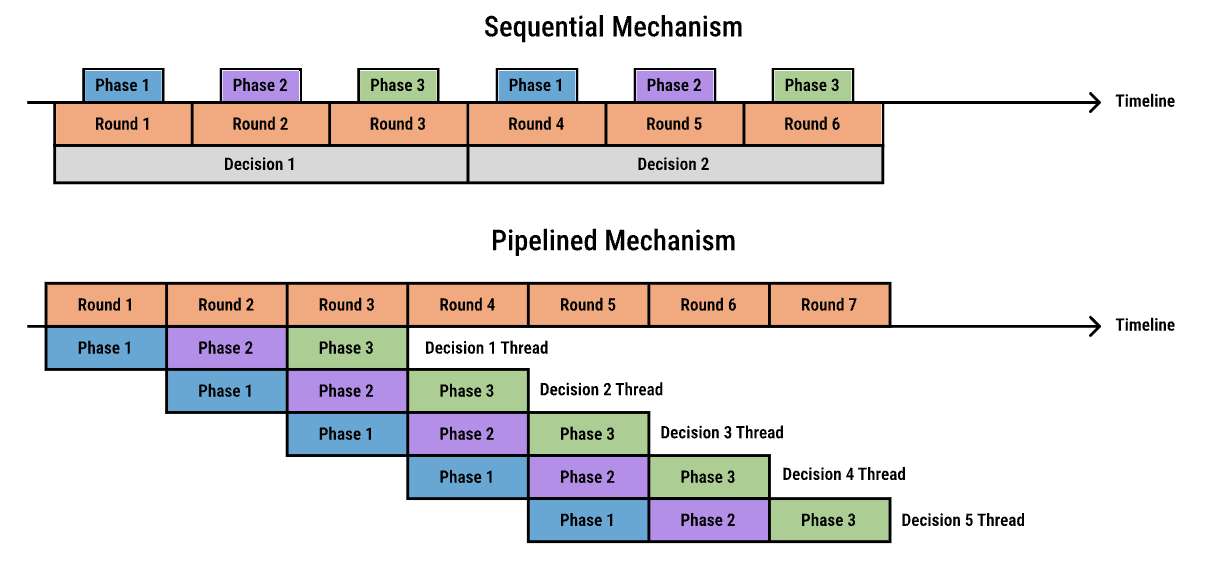
\includegraphics[width=3.4in]{pipeline_mechanism.pdf}
% \caption{Pipelined execution: the phases of several agreement instances
% overlap on a chain of deterministic flood rounds.}
% \label{fig:pipeline}
% \end{figure}

A conventional agreement protocol serialises its phases: the system waits
until a proposal has been disseminated network-wide and the votes of all
nodes have been collected before the next decision may begin. Every node
is idle for most of that interval, and throughput is bounded by the
round-trip structure of a single instance rather than by the capacity of
the medium.

We remove that constraint by allowing nodes to inject new proposals and
votes without waiting for earlier instances to complete. Because the
terminating slot of every flood round is known in advance, an initiator
can use its turn to advance several instances at once: in a single round
it carries the state of instance $k-1$, which may be in its commit phase,
and simultaneously piggybacks the proposal or vote belonging to instance
$k$, which is entering its first phase. Under sustained load the network
is therefore always advancing several phases of several different
agreements concurrently, and the medium is never idle waiting for a
round trip to close.

It is worth distinguishing this from batching, with which it is easily
confused (Section~\ref{sec:back-pipelining}). Batching would enlarge the
payload of one instance; pipelining overlaps distinct instances, so a
proposal may enter in any round instead of waiting for the current batch
to close, and the latency of an individual decision is unaffected. The
number of instances concurrently in flight, which we call the pipeline
depth $\Cdepth$ and quantify in Section~\ref{sec:results}, is accordingly
not a tuning parameter but a consequence of the ratio between the phase
structure of the protocol and the round length of the substrate.

%%---------------------------------------------------------------------
\subsection{Preserving Total Order and Constructive Interference}
\label{sec:design-order}

Pipelining an agreement protocol over \CI{} raises an immediate physical
objection. Constructive interference requires that concurrent
transmitters emit bit-identical packets in the same slot
\cite{ferrari11glossy}; if several decisions are in flight and nodes hold
differing views of them, the packets they relay could differ and the
superposition would be destructive rather than constructive. The design
resolves this by keeping content generation and content relaying strictly
separate.

Within a round, only the initiator of that round generates content; every
other node retransmits the received bytes verbatim, exactly as in a
standard \CI{} flood. No node modifies a packet in flight, and the
physical requirement is therefore satisfied by construction, independently
of how many instances are in progress. Local state influences the network
only at the moment a node's own turn arrives: at that point the node
determines, from the order in which it received the messages of previous
rounds, where each proposal and vote belongs in the payload it is about to
transmit.

The correctness argument follows from the determinism established in
Section~\ref{sec:model-timing}. That ordering is derived from the same
fixed sequence of completed rounds at every node, so all nodes that are
up to date reach identical conclusions about the contents of the next
packet, and the relays of the following round consequently reproduce a
bit-identical frame. Total order is thus not enforced by an additional
protocol layer; it is inherited from the slot timing of the substrate. In
contrast to \CE-based designs, where concurrency and ordering are in
direct conflict, here concurrency is safe precisely because nothing is
merged in flight.

%%---------------------------------------------------------------------
\subsection{Unified Message Format}
\label{sec:design-format}

% TODO: uncomment once figures/message_frame.pdf exists.
% \begin{figure}[!t]
% \centering
% 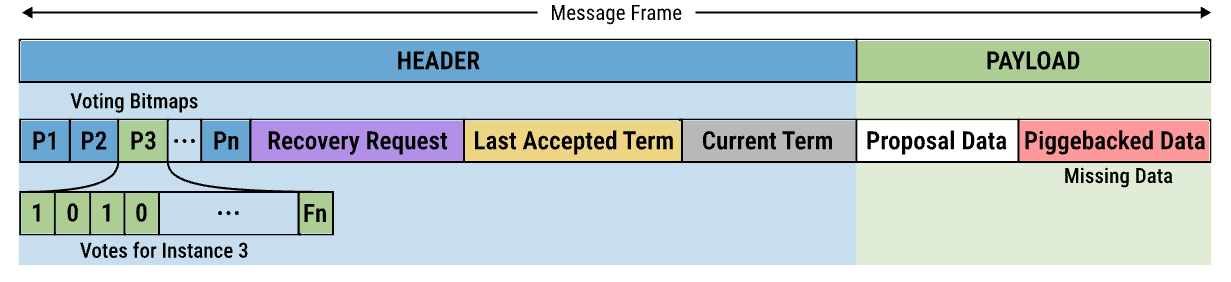
\includegraphics[width=3.4in]{message_frame.pdf}
% \caption{Unified frame format: a control header (term identifier, last
% accepted term, participation bitmap and NACK field) followed by the
% pipelined payload.}
% \label{fig:frame}
% \end{figure}

Low-power radios impose tight frame budgets, so pipelining and state
recovery must share one compact structure rather than each introducing its
own control traffic. The frame has two parts: a control header that drives
the state machine, and a payload that carries protocol content.

\subsubsection{Control header}
The header carries four fields.

\begin{itemize}
\item \textbf{Term identifier.} A monotonically increasing counter
locating the current decision in the global sequence. A node detects a gap
in its log by comparing this field against its own last recorded value,
without hashing or any other non-trivial computation.

\item \textbf{Last accepted term.} The identifier of the most recent
decision the sender has finalised. Because decisions are sequential, this
single field acknowledges that decision and every decision preceding it,
which is what allows commit notifications to occupy no payload space at
all.

\item \textbf{Participation bitmap.} A field of $\Nnodes$ bits, one per
node. On receiving a frame---whether addressed to it or merely
overheard---a node sets its own bit to record its acknowledgement or
affirmative vote, so that votes accumulate across the network without any
dedicated acknowledgement message.

\item \textbf{NACK field.} Zero in normal operation. A node that infers
from the term identifier that it has fallen behind writes the identifier
of its last successful decision here, thereby requesting recovery.
\end{itemize}

\subsubsection{Pipelined payload}
The payload holds the proposal data requiring agreement, followed by
piggybacked pipeline data: the state of the preceding transaction, or the
content requested by an outstanding NACK. This is the field that makes
the overlap of Section~\ref{sec:design-pipeline} concrete, and it is also
what allows a lagging node to be brought up to date without interrupting
the pipeline, since recovery data travels in the same frames that carry
new decisions forward.

\subsubsection{Frame size and scalability}
The only component of the header that grows with the network is the
bitmap, at one bit per node: for the $\Nnodes = 27$ network used
throughout Section~\ref{sec:results} it occupies four bytes, which is
negligible beside the payload capacity available on the Bluetooth~5
physical layers targeted by BlueFlood \cite{alnahas21blueflood}. We note
for completeness that this linear growth bounds the design: at several
hundred nodes the bitmap would begin to compete with the payload for frame
space, and a coarser representation would be required. We have not
evaluated such a representation, and the networks studied here are far
from that regime.

%%---------------------------------------------------------------------
\subsection{Protocol Instantiations}
\label{sec:design-protocols}
We instantiate three standard agreement protocols on the pipeline
described above. They are chosen deliberately: they span the space of
agreement conditions, requiring respectively a majority quorum, unanimity,
and no vote at all. Because they share a substrate, a schedule and a frame
format, and differ only in that condition, the comparison in
Section~\ref{sec:results} isolates the effect of the agreement condition
itself.

%%---------------------------------------------------------------------
\subsubsection{Paxos}
\label{sec:design-paxos}

% TODO: uncomment once figures/paxos_ci_example.pdf exists.
% \begin{figure}[!t]
% \centering
% 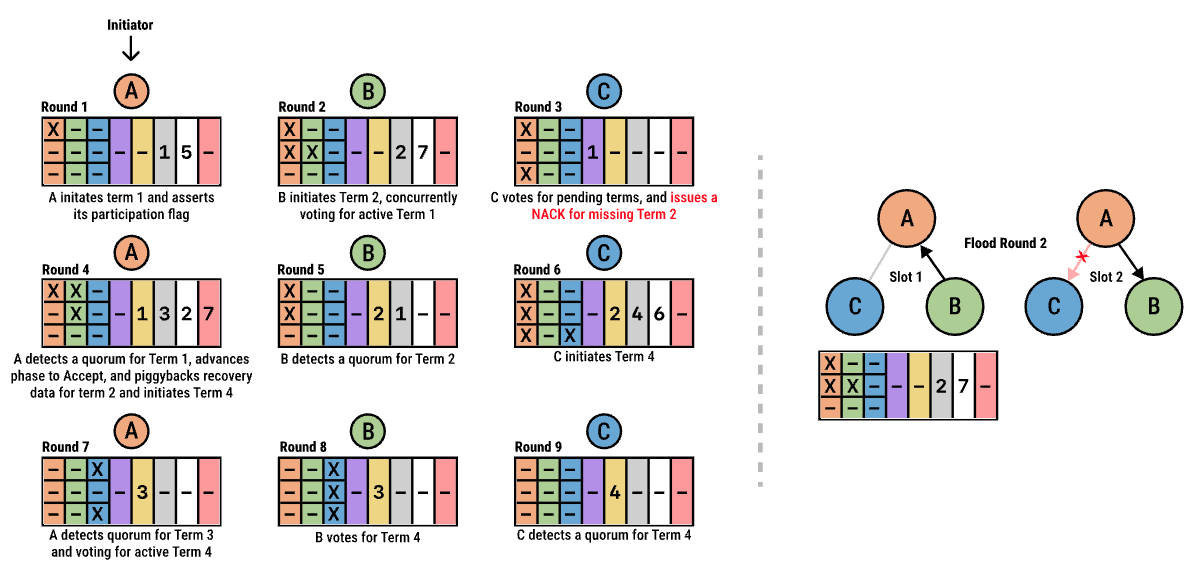
\includegraphics[width=3.4in]{paxos_ci_example.pdf}
% \caption{Pipelined Paxos over \CI: implicit vote aggregation through the
% participation bitmap and cumulative acknowledgement through the last
% accepted term.}
% \label{fig:paxos}
% \end{figure}

Combining Paxos with the round-robin schedule removes several of the
costs that the protocol incurs in an asynchronous setting. As established
in Section~\ref{sec:design-rounds}, the term space is partitioned among
nodes in advance, so two proposers can never contend for the same term.
Proposal collision is therefore structurally impossible, and the classical
Promise phase---whose purpose is to reserve a ballot number and discover
contention---is redundant and omitted. Agreement proceeds as a continuous
pipelined cycle in four steps.

\paragraph{Proposal initiation}
When the turn of node $i$ arrives, it opens a new agreement instance: it
fixes the current term identifier, places its value in the proposal field,
and initiates the flood.

\paragraph{Implicit, concurrent quorum}
Instead of soliciting dedicated acknowledgements, the protocol relies on
overhearing. Every node that receives the frame sets its own bit in the
participation bitmap, so votes accumulate as the schedule advances through
the remaining nodes of the cycle. Since a frame carries the bitmaps of
several instances at once, nodes evaluate the state of several
in-flight decisions in parallel, and no instance has to be suspended while
another collects its votes.

\paragraph{Cumulative commit}
When the turn returns to the original proposer, it inspects the bitmap and
determines whether a majority quorum has been reached. If so, it does not
spend a frame on a dedicated Accept message: it simply advances the last
accepted term field of its next header. Because decisions are sequential,
that single field implicitly informs the whole network that this
transaction and all preceding ones are final, leaving the payload free to
carry the pipeline forward.

\paragraph{Non-blocking recovery}
A node that misses frames during a transient link outage does not stall
the network. On receiving the next frame it compares the term identifier
and last accepted term against its local history and immediately detects
the gap, then writes the missing identifier into the NACK field. In
subsequent rounds, nodes that are up to date append the missing content to
the piggybacked recovery portion of their own frames. Recovery thus
proceeds in the background, in the same frames that carry new decisions,
and the pipeline never blocks on a lagging node.

%%---------------------------------------------------------------------
\subsubsection{Non-Blocking Two-Phase Commit}
\label{sec:design-2pc}

Two-phase commit resembles Paxos in message flow but requires unanimity to
proceed, which in wireless settings has historically made it fragile:
a single unreachable participant forces the system into long, blocking
timeouts. Instantiating it on a deterministic pipeline neutralises this
structurally.

\paragraph{Transaction initiation}
When the turn reaches the node acting as coordinator for a new
transaction, it writes the transaction identifier into the header, sets
the phase indicator to Prepare, and floods the transaction data.

\paragraph{Deterministic, bounded voting}
The voting window is not a timeout to be tuned but a structural quantity:
it is exactly one cycle, that is $\Nnodes$ rounds, during which every node
takes its turn once. Each node evaluates the transaction and, if it can
commit, sets its bit in the participation bitmap. The volatile, poorly
conditioned timeouts of conventional 2PC disappear entirely. The
sufficiency of this bound depends on the ratio of diameter to network
size; Section~\ref{sec:results} shows that it does not hold when $\Diam$
approaches $\Nnodes$, and treats that case as a limitation of the present
design.

\paragraph{Distributed decision}
Thanks to overhearing, the accumulated bitmap is replicated at every node.
The decision is consequently not taken by the coordinator: once exactly
one cycle has elapsed since the transaction opened, \emph{each node}
independently evaluates the bitmap. Unlike Paxos, a node commits only if
every bit is set; a single clear bit---whether from a negative vote or
from an unreachable node---yields abort. Since the input to this
evaluation is the same replicated bitmap and the instant of evaluation is
the same deterministic bound, all informed nodes reach the same verdict
independently and without further communication. An explicit negative vote
is in addition propagated as an abort flag, which terminates the
transaction immediately rather than at the end of the window.

\paragraph{Non-blocking execution}
In conventional 2PC, failure of the coordinator after votes have been
collected blocks the participants indefinitely; three-phase commit
addresses this by inserting an additional pre-commit phase, at the cost of
an extra round trip \cite{skeen81nonblocking}. The present design achieves
the same property without a third phase, and the reason lies in the
preceding step: because every node holds the complete bitmap and decides
independently at a shared deterministic instant, \emph{no node waits for a
message from the coordinator in order to finalise the transaction}.
Failure of the initiating node therefore blocks nobody, and no
coordinator election is required---there is no centralised decider to
replace. The result is the reliability of 3PC at the message cost of 2PC,
with the pipeline kept continuously in motion. As stated in
Section~\ref{sec:model-fault}, this is a structural argument; crash
failures are not simulated in this paper.

%%---------------------------------------------------------------------
\subsubsection{Total-Order Multicast}
\label{sec:design-tom}

Total-order multicast requires that all nodes deliver messages to the
application in an identical order. Classical implementations obtain this
from a central sequencer, which becomes both a throughput bottleneck and a
single point of failure \cite{defago04total}. The deterministic rotation
of the substrate makes the sequencer unnecessary.

\paragraph{Distributed, deterministic sequencing}
The round-robin schedule is itself a distributed sequencer. When the turn
reaches node $i$, that node increments the global term identifier by one
and transmits. Because injection is tied to predetermined slots, messages
enter the network in a strictly monotonically increasing order by
construction, with no coordination whatsoever.

\paragraph{In-order delivery}
Since \CI{} flooding admits none of the reordering anomalies of
multi-path routing, messages arrive in the order in which they were
issued. The middleware at each node delivers a message to the application
only when its term identifier is exactly one greater than that of the last
delivered message.

\paragraph{Tolerating sequencer failure}
If the node whose turn it is has crashed, or simply has nothing to send,
the network does not stall and no election takes place: its slot elapses
and the turn passes to the next node, which continues the sequence from
the last successful term. The vulnerability of the classical sequencer to
point failures thus disappears.

\paragraph{Gap detection and catch-up}
Preserving total order under packet loss is the central difficulty of
TOM. Here a node that misses a message detects the sequence gap on
receiving the next one, buffers subsequent messages locally instead of
delivering them, and writes the missing term into the NACK field. Other
nodes observing the request retransmit the missing message in the
recovery portion of their frames. Once the gap is filled, the node
processes its buffer in term order and rejoins the pipeline. This
mechanism preserves correctness, but it makes delivery latency sensitive
to head-of-line blocking on long paths, an effect quantified in
Section~\ref{sec:results}.


\section{Capture-Effect Baseline}
\label{sec:baseline}
To place the results of Section~\ref{sec:results} in context we require a
baseline that represents the state of the art rather than a weakened
version of it. Agreement over the capture effect is that baseline: it is
the mechanism underlying Chaos, A2/Synchrotron and Wireless Paxos, the
systems that established that agreement over synchronous transmissions is
feasible at all \cite{landsiedel13chaos}, \cite{alnahas17a2},
\cite{poirot19paxos}. This section describes how it attains its
efficiency, and then why that same mechanism confines it to one decision
per round. The limitation we identify is structural, not an artefact of
any particular implementation.

%%---------------------------------------------------------------------
\subsection{In-Network Merging}
\label{sec:baseline-merge}

Under the capture effect, a receiver exposed to several concurrent
transmissions decodes the strongest of them, provided its power exceeds
the others by a hardware-dependent margin and arrives within the
receiver's synchronisation window \cite{wilhelm14reception}. The packets
need not be identical, and this is what the baseline exploits: nodes do
not relay bytes verbatim but merge the state they receive with the state
they hold, typically by an idempotent, commutative and associative
operator such as a bitwise union of vote or participation vectors, before
retransmitting the result \cite{landsiedel13chaos}.

The consequence is that the flood is no longer transport but computation.
Each hop performs part of the aggregation, so the number of slots required
to collect an aggregate over the whole network grows far more slowly than
the number of nodes, and agreement is reached without any node ever
transmitting an individual report. This is a genuinely strong design:
A2 completes two-phase commit across 180 nodes in 475\,ms
\cite{alnahas17a2}, and Wireless Paxos reaches consensus among 188 nodes
in 289\,ms \cite{poirot19paxos}. Any claim of improvement must be measured
against these figures, and Section~\ref{sec:method} accordingly calibrates
the baseline against them rather than against an idealised model.

%%---------------------------------------------------------------------
\subsection{The Sequential Limit}
\label{sec:baseline-sequential}

The merging step is also the source of the limitation. Because content is
rewritten in flight, the packet observed at a given point in the network
depends on which nodes it has already traversed. With a single decision in
progress this is harmless, since the aggregation operator is order
insensitive and all nodes converge on the same aggregate. With two
decisions in progress it is not: an operator that is commutative by
construction cannot record which proposal was issued first, so concurrent
proposals merge into an unordered set from which no total order can be
recovered. Overlapping instances would therefore not merely degrade
performance, they would violate the ordering guarantee that the protocols
exist to provide. \CE-based designs consequently enforce a
one-decision-per-round rule, and every proposal arriving during a round
must wait for the next one.

A second consequence concerns energy, and it follows from the termination
condition rather than from the merge operator. A \CE{} round ends when a
goal has been achieved network-wide, which no node can predict in advance;
rounds are therefore bounded by timeouts and every node must keep its
radio active for the entire round in case a relevant transmission still
arrives. The radio-on cost of a round is accordingly

\begin{equation}
\label{eq:ece}
\Ece \;=\; \Nnodes \cdot \Lround ,
\end{equation}

that is, the full product of network size and round length, with no
opportunity to sleep. Under \CI{} the corresponding cost is bounded by
Equation~\eqref{eq:round}: because the terminating slot is known in
advance, a node that has completed its retransmission duty may power its
radio down for the remainder of the round.

These two properties compound. The baseline pays the full energy of a
round for exactly one decision, whereas the pipeline of
Section~\ref{sec:design} amortises a comparable cost over several
decisions in flight; Section~\ref{sec:results} quantifies the resulting
gap. We stress that Equation~\eqref{eq:ece} describes a design that is
efficient by the standards of its own model, and that the comparison in
this paper is deliberately generous to it: as Section~\ref{sec:method}
records, the baseline is granted idealised capture behaviour, so its
reported performance is an upper bound on what the mechanism can achieve
in practice.


\section{Evaluation Methodology}
\label{sec:method}
We evaluate the proposed architecture against the capture-effect baseline
of Section~\ref{sec:baseline} under identical conditions, with the aim of
characterising scalability, convergence speed and resource efficiency
across a range of traffic regimes.

%%---------------------------------------------------------------------
\subsection{Implementation and Simulation Environment}
\label{sec:method-env}

Evaluating these protocols requires faithful reproduction of link-layer
behaviour, exact slot timing, and the state machines of three distributed
protocols. We therefore conducted all experiments in a custom slot-level
discrete-event simulator written in Rust, chosen for its performance,
memory safety and type system, which together allow each node to be
modelled as an independent entity while keeping large numbers of
communication rounds tractable. The simulator advances one slot at a
time; in every slot the radio state of every node---listening, flooding,
or asleep---is recorded and the corresponding energy counters are updated.
Energy is thus not estimated from an analytical model but accumulated
directly from the simulated radio schedule.

Both communication substrates were implemented from scratch in the same
environment: the capture-effect mechanism after the Chaos model
\cite{landsiedel13chaos} and the constructive-interference mechanism after
the BlueFlood model \cite{alnahas19blueflood}, as were all six protocol
variants (2PC, TOM and Paxos, each over \CI{} and over \CE). Sharing an
implementation, a scheduler and an energy accounting path in this way
isolates the comparison from differences in engineering quality, which is
the principal confound when results obtained on different codebases are
placed side by side. Simulator logs were post-processed with Python using
Pandas and NumPy, and figures were produced with Matplotlib and Seaborn.

%%---------------------------------------------------------------------
\subsection{Experimental Parameters and Network Model}
\label{sec:method-params}

Scenarios were generated by varying four parameters.

\begin{itemize}
\item \textbf{Network size ($\Nnodes$).} From small deployments
($\Nnodes = 6$) to $\Nnodes = 188$, the latter matching the largest
configuration reported for Wireless Paxos \cite{poirot19paxos} so that
our figures can be read against the published ones.

\item \textbf{Topology.} Five multi-hop topologies spanning a wide range
of diameters: full mesh ($\Diam = 1$), partial mesh ($\Diam = 3$), random
($\Diam = 4$), scale-free ($\Diam = 4$) and line ($\Diam = 26$). Random
and scale-free are matched in diameter (Table~\ref{tab:topologies}) but
differ in the shape of their degree distribution, a pair chosen deliberately
to test whether diameter alone predicts behaviour.

\item \textbf{Loss model.} Independent and identically distributed packet
loss on each link, swept from 0\,\% to 20\,\%, as specified in
Section~\ref{sec:model-fault}.

\item \textbf{Workload.} 100 proposals per run. Every reported data point
is the mean of fifteen independent random seeds.
\end{itemize}

Unless stated otherwise, the reference operating point throughout
Section~\ref{sec:results} is a 27-node network with random topology
($\Diam = 4$) and 5\,\% link loss.

%%---------------------------------------------------------------------
\subsection{Evaluation Metrics}
\label{sec:method-metrics}

Four primary metrics are extracted from the logs, together with one
derived quantity.

\begin{itemize}
\item \textbf{Throughput.} The number of proposals reaching a final,
network-wide decision per slot. This is the metric on which the claim of
Section~\ref{sec:design} stands or falls, since it is where pipelined and
sequential processing are expected to diverge under load.

\item \textbf{Decision latency.} The number of slots elapsed between the
initiator issuing a proposal and the network completing agreement on it.
We report it separately from throughput because, as
Section~\ref{sec:results} shows, the two need not move together in a
pipelined system.

\item \textbf{Awake slots.} The total number of slots in which a node's
radio was transmitting, receiving or listening. In low-power wireless,
radio-on time is the dominant contributor to energy consumption, and the
distribution of this quantity across nodes indicates how evenly that cost
is borne. Two run lengths must be distinguished, because they differ whenever
the pipeline drains. $\Send$ is the slot at which the last decision commits,
and throughput and pipeline depth are per $\Send$; $\Ssim$ is the total number
of slots ticked, and energy is per $\Ssim$. Under \CE{} the two coincide in
every measurement reported here. Under \CI{} they differ by the drain tail,
by $0.09\,\%$ for TOM, $1.70\,\%$ for Paxos and $3.41\,\%$ for 2PC at the
reference point, reaching $23.4\,\%$ on a single seed.

\item \textbf{Commit rate.} The fraction of the offered workload that
reaches a definitive global decision. This metric exposes the robustness
of each architecture's recovery machinery under loss, and it is the
metric that reveals the design limitation reported in
Section~\ref{sec:results}.
\end{itemize}

Finally, we characterise concurrency itself. The mean number of agreement
instances simultaneously in flight, the pipeline depth introduced in
Section~\ref{sec:design-pipeline}, is not measured directly but obtained
from the two primary metrics by Little's law,

\begin{equation}
\label{eq:depth}
\Cdepth \;=\; \text{Throughput} \times \text{Latency} .
\end{equation}

Reporting $\Cdepth$ matters because throughput and latency alone cannot
distinguish a system that is fast from one that is concurrent;
Equation~\eqref{eq:depth} separates the two, and the value it yields for
the baseline is the quantitative statement of the one-decision-per-round
rule.

%%---------------------------------------------------------------------
\subsection{Simulator Validation and Scope of Abstraction}
\label{sec:method-validation}
All results in this paper are obtained in simulation, so the weight a
reader may place on them depends on what the abstraction does and does not
reproduce. This subsection states that explicitly. We adopt the standard
terminology, in which verification asks whether the model is implemented
correctly and validation asks whether it is adequate \emph{for its
intended purpose} \cite{sargent13validation}. The purpose here is
comparative: every claim we make concerns the relative behaviour of two
architectures evaluated on a shared substrate model, shared scheduler and
shared energy accounting, not the absolute performance of either on
specific hardware. Validation is organised in three layers, each
addressing a different way in which such a comparison could fail.

\subsubsection{Layer 1: internal and analytical consistency}
The first layer checks the implementation against closed-form properties
that the design predicts independently of any measurement. Observed round
lengths must equal $\Diam + \Nretx$ slots for every topology, per
Equation~\eqref{eq:round}; the radio-on cost of the baseline must satisfy
the identity $\Ece = \Nnodes \cdot \Lround$ of
Equation~\eqref{eq:ece}, which Section~\ref{sec:results} confirms exactly
across fifteen configurations; per-node radio state
counters must sum to the aggregate energy totals; and no decision may be
reported as committed unless the corresponding quorum condition is
satisfied in the recorded bitmaps. These are necessary conditions, and we
note plainly that they test the code rather than the abstraction: a model
that is internally consistent may still rest on unrealistic physical
assumptions.

\subsubsection{Layer 2: cross-level calibration against published measurements}
The second layer addresses precisely that risk, and it is the layer on
which the credibility of the results principally rests. It proceeds in two
steps that must not be conflated.

In the calibration step, the physical abstraction has one free parameter
and one target. The per-attempt loss-rate upper bound is frozen at
$p^*=0.05$ against BlueFlood's published end-to-end flood coverage over
receivers of approximately 99.9\,\%
\cite{alnahas19blueflood}, \cite{alnahas21blueflood}. The target ``radio duty
cycle $\sim$0.4\,\%'' was dropped before calibration because its wall-clock
denominator includes inter-round idle time that the simulator does not
model. The slot duration $\Tslot$ is instead a paper-side unit conversion,
not a second calibrated parameter.

The prediction step freezes that parameter and tests two published results
that played no part in calibration. At the pre-registered
$T_{\mathrm{guard}}=10\,\mu\mathrm{s}$ acceptance point, A2 predicts
16.722\,ms [16.527, 16.917] against 475\,ms (relative error $-0.9648$), while
Wireless Paxos predicts 9.796\,ms [9.735, 9.858] against 289\,ms (relative
error $-0.9661$). These are blind predictions, not fits: both fail the
acceptance test at every $T_{\mathrm{guard}}$ from 10 to 100\,$\mu$s, with
the pre-registered-point errors reported as $-96.5\,\%$ and $-96.6\,\%$.
The distinct raw-slot comparison gives 42.441 slots [41.946, 42.935] for A2,
outside its pre-registered slot-equivalent interval [828, 1205], and 24.614
slots [24.459, 24.769] for Wireless Paxos, outside [500, 726]. The failed
predictions therefore reject cross-level agreement with the published
testbed latencies rather than validating it. All three profiles remain
regression tests so that the frozen calibration cannot silently drift.

\subsubsection{Layer 3: sensitivity and invariance}
The third layer asks whether the conclusions survive perturbation of the
abstraction itself. We sweep the number of retransmissions $\Nretx$, the
slot duration $\Tslot$, and the loss process---replacing the
independent model of Section~\ref{sec:model-fault} with a correlated,
bursty one---and verify that the ordering of the architectures does not
invert. What matters for a comparative claim is not that the numbers are
reproduced exactly under every assumption, but that the sign of the
difference is stable; we report the range over which it holds. The topology
sweep of
Section~\ref{sec:results}, spanning diameters from 1 to 26, is itself an
invariance test of this kind, and it is also where the one regime we have
found in which a pipelined protocol is not competitive comes to light.

\subsubsection{Scope of abstraction and direction of bias}
Several phenomena are deliberately excluded from the model. Rather than
list them as caveats, we state for each one the direction in which it
biases the comparison, since an omission that favours the baseline
strengthens our claims while one that favours the proposed architecture
weakens them. Table~\ref{tab:bias} summarises the analysis.

\begin{table}[!t]
\caption{Excluded phenomena and the direction in which each biases the
comparison between the proposed architecture and the baseline.}
\label{tab:bias}
\centering
\begin{tabular}{@{}p{0.33\columnwidth}p{0.17\columnwidth}p{0.38\columnwidth}@{}}
\toprule
\textbf{Excluded phenomenon} & \textbf{Favours} & \textbf{Treatment} \\
\midrule
Idealised capture behaviour in the \CE{} baseline &
Baseline &
Left in place; the baseline is reported at an upper bound, so the
comparison is conservative \\
\addlinespace
\CI{} synchronisation assumed always to succeed &
Proposed &
Offset by fixing the loss rate to the measured BlueFlood delivery ratio
(Layer~2) \\
\addlinespace
Clock drift between floods &
Proposed &
Bounded by published drift measurements and absorbed by the guard band
\cite{baddeley23understanding} \\
\addlinespace
MCU processing and cryptographic delay &
Neither &
Identical in both architectures; cancels in the comparison \\
\addlinespace
Correlated (bursty) packet loss &
Unknown &
Examined in the Layer~3 sensitivity sweep \\
\addlinespace
Node crash failures &
Neither &
Out of scope by Section~\ref{sec:model-fault} \\
\bottomrule
\end{tabular}
\end{table}

Two entries deserve comment. The idealised capture assumption is the one
exclusion we make no attempt to correct: real capture requires a power
margin and a narrow arrival window, and it fails more often than our model
admits \cite{wilhelm14reception}, so the baseline as simulated performs at
least as well as a real deployment would. The assumption that \CI{}
synchronisation always succeeds cuts the other way, and it is the reason
the Layer~2 calibration matters: by tying the loss rate to a measured
delivery ratio, the optimism of the synchronisation model is absorbed
into an empirically grounded loss process rather than left free.

Accordingly, we do not claim absolute latency or energy figures
transferable to a particular platform, nor any result concerning
performance under crash or Byzantine faults. What the evaluation supports
is a comparison, under stated and bounded assumptions, between two
architectures that differ in exactly one respect: whether agreement
instances may overlap.


\section{Results}
\label{sec:results}
This section analyses the behaviour of the three protocols on both
communication substrates. Before turning to the individual metrics,
Table~\ref{tab:baseline} summarises the reference operating point defined
in Section~\ref{sec:method-params}: 27 nodes, random topology of diameter
4, 5\,\% link loss, 100 proposals, each figure the mean of fifteen seeds.

\begin{table}[!t]
\caption{Summary at the reference operating point ($\Nnodes = 27$, random
topology, 5\,\% loss). Thr.\ = committed decisions per slot; Lat.\ = mean
slots per decision; $E$/dec = listening and flooding slots per committed
decision; Eff.\ = $1000 \times$ (throughput / energy per decision);
Sleep = total node sleep slots.}
\label{tab:baseline}
\centering
\footnotesize
\setlength{\tabcolsep}{4pt}
\begin{tabular}{@{}lrrrrrr@{}}
\toprule
\textbf{Protocol} & \textbf{Commit} & \textbf{Thr.} & \textbf{Lat.} &
\textbf{$E$/dec} & \textbf{Eff.} & \textbf{Sleep} \\
 & (\%) & & & & & \\
\midrule
TOM (\CI)   & 100.0 & 0.2132 & 4.7   & 88.0  & 2.429 & 3900 \\
Paxos (\CI) & 100.0 & 0.1903 & 61.4  & 100.2 & 1.906 & 4434 \\
2PC (\CI)   & 98.9  & 0.1681 & 126.8 & 115.8 & 1.463 & 5034 \\
\addlinespace
TOM (\CE)   & 100.0 & 0.2143 & 4.7   & 126.3 & 1.705 & 0 \\
Paxos (\CE) & 100.0 & 0.0704 & 14.2  & 383.6 & 0.184 & 0 \\
2PC (\CE)   & 100.0 & 0.0412 & 24.3  & 657.1 & 0.063 & 0 \\
\bottomrule
\end{tabular}
\end{table}

The table places all four metrics of Section~\ref{sec:method-metrics}
side by side deliberately, because the central finding of this work lies
not in any single column but in the tension between them. For TOM, the
two substrates are indistinguishable in speed: 0.2132 against 0.2143
decisions per slot, both at 4.7 slots of latency. Yet even at equal
speed the energy efficiency clearly favours \CI{} (2.43 against 1.70),
and the Sleep column identifies the reason. It is exactly zero for all
three \CE{} protocols---no radio is ever switched off for the duration of
the run---whereas the \CI{} architecture spends a substantial fraction of
all node-slots asleep. This is Equation~\eqref{eq:ece} made visible.

For the vote-based protocols the pattern differs. The \CI{} variants are
far ahead on throughput and efficiency despite latencies several times
higher: 2PC over \CI{} takes 126.8 slots per decision against 24.3 for
its \CE{} counterpart, yet delivers more than four times the throughput
and more than twenty times the efficiency. The commit-rate column shows
that at this operating point the architectural difference does not
generally manifest as transaction failure; only 2PC over \CI{} falls
slightly short of complete commitment, at 98.9\,\%, which is a
consequence of the bounded voting window that unanimity requires
(Section~\ref{sec:design-2pc}) and is examined below.

The subsections that follow open up each of these columns over a wider
range of network sizes, loss rates and topologies.

%%---------------------------------------------------------------------
\subsection{Throughput and Scalability}
\label{sec:results-throughput}

Throughout this subsection throughput is the ratio of committed decisions
to the total number of slots elapsed until the workload completes, with
all-node completion as the termination criterion. Shaded bands in the
figures show the spread across seeds.

\subsubsection{Effect of network size}

% TODO: uncomment once figures/throughput_vs_nodes.pdf exists.
% \begin{figure}[!t]
% \centering
% 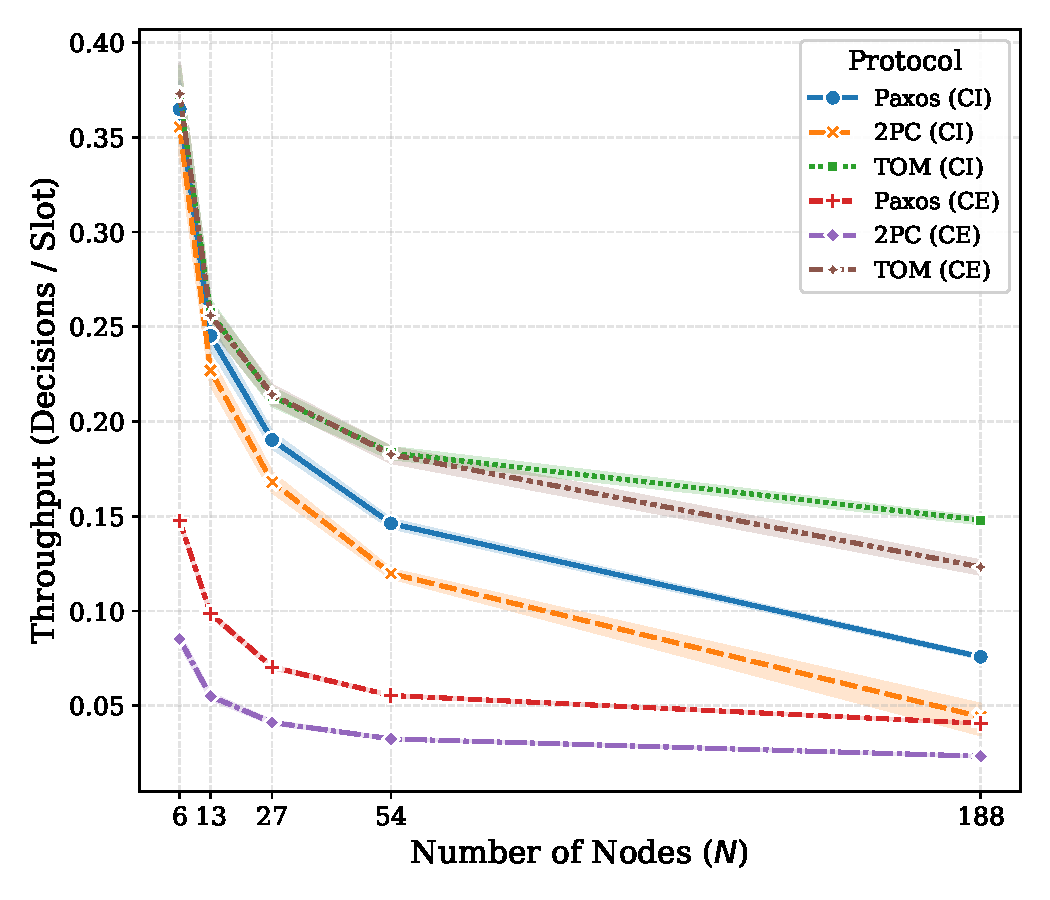
\includegraphics[width=3.4in]{throughput_vs_nodes.pdf}
% \caption{Throughput (decisions per slot) against network size
% $\Nnodes$ at 5\,\% link loss (random topology, 100 proposals; mean
% $\pm$ spread across seeds).}
% \label{fig:thr-nodes}
% \end{figure}

Throughput falls with $\Nnodes$ for every protocol, since the diameter
and hence the length of each flood round grows, and more nodes must be
reached before all-node completion holds. The slopes differ, however, and
those differences expose the interaction between the communication
architecture and the structure of the protocol.

The decisive observation is that the curves separate into two clusters
whose boundary is \emph{not} the boundary between \CI{} and \CE. The
upper cluster contains all three \CI{} protocols together with TOM over
\CE; the lower contains only Paxos and 2PC over \CE. The gap between them
is large: at $\Nnodes = 27$ the weakest member of the upper cluster, 2PC
over \CI{} at 0.168, still produces more than twice the decisions of the
strongest member of the lower cluster, Paxos over \CE{} at 0.070. What
relegates a combination to the lower cluster is therefore the sequential
execution of a multi-phase protocol, not the choice of physical layer as
such.

Among the vote-based protocols the advantage of pipelining is stable
across every network size. At $\Nnodes = 27$, Paxos over \CI{} achieves
roughly 2.7 times and 2PC over \CI{} roughly four times the throughput of
their \CE{} counterparts. This is obtained \emph{despite} the higher
per-decision latency of the \CI{} variants documented in
Section~\ref{sec:results-latency}, and its origin is the overlap of
several proposals on one shared chain of flood rounds: the pipeline
amortises the fixed temporal cost of rounds across concurrent
transactions and thereby raises the rate at which the workload as a whole
completes.

TOM behaves differently, and instructively. In small and medium networks
the two TOM curves lie almost exactly on top of one another
(0.213 against 0.214 at $\Nnodes = 27$), neither substrate holding an
advantage. This coincidence is not accidental and has a structural
explanation, quantified in Section~\ref{sec:results-dynamics}. As the
network grows the curves diverge: from $\Nnodes = 54$ onward TOM over
\CI{} pulls ahead, and at $\Nnodes = 188$ its throughput is about 20\,\%
higher (0.148 against 0.123). The fixed cost of \CI{} rounds becomes less
significant relative to path length as the diameter grows, while \CE{}
faces increasing contention and sequential merging as nodes are added.

At the bottom of the ranking, 2PC over \CE{} has the lowest throughput at
every network size: unanimity combined with strictly sequential execution
is the most expensive point in the design space we examine.

\subsubsection{Resilience of throughput to packet loss}

% TODO: uncomment once figures/throughput_vs_loss.pdf exists.
% \begin{figure}[!t]
% \centering
% 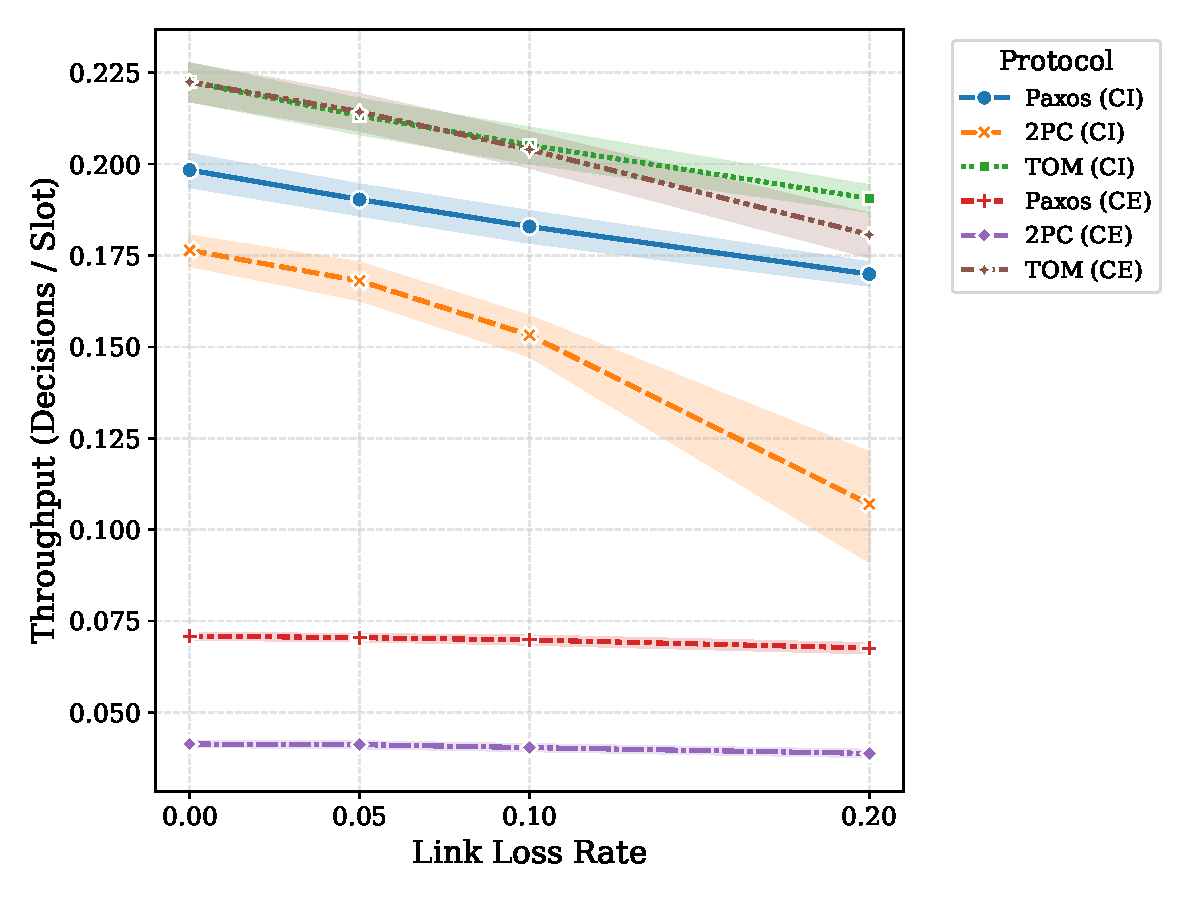
\includegraphics[width=3.4in]{throughput_vs_loss.pdf}
% \caption{Throughput against link loss rate for $\Nnodes = 27$ (random
% topology, $\Diam = 4$, 100 proposals).}
% \label{fig:thr-loss}
% \end{figure}

Raising the loss rate from 0 to 20\,\% degrades most protocols gently.
TOM on both substrates and Paxos over \CI{} lose between 15\,\% and
19\,\% of their throughput across that range and their curves remain
close to linear. Both pure dissemination and the majority condition are
thus inherently loss-tolerant: in the first case neighbouring
retransmissions compensate for a missing copy, and in the second reaching
a quorum does not require every node to participate.

The most sensitive combination is 2PC over \CI. Its throughput tracks the
others up to 10\,\% loss and then falls considerably more steeply, to
about 0.107---some 39\,\% below its lossless value---while the spread
across seeds widens noticeably. The explanation lies in the interaction
between unanimity and the fixed pipeline window: losing the vote of even
one node makes the unanimity condition hard to satisfy within the
allotted window, so the transaction is either carried into later rounds
or aborted. Because pipeline resources are shared, every stalled
transaction also consumes slots that later proposals would have used, and
the effect of a loss propagates through the pipeline. The widening
confidence band reflects exactly this sensitivity to the random pattern
of losses.

The curves for Paxos and 2PC over \CE, by contrast, remain almost
perfectly flat at a low level, declining by only 4--5\,\% over the whole
range. This should not be read as superior robustness. These protocols
have already reached their structural bottleneck through sequential
execution and an always-on radio, and adding channel errors changes
little relative to that dominant constraint; the fixed architectural
overhead is large enough to hide the channel noise behind it.

It is worth noting that even at its worst operating point---20\,\% loss
---2PC over \CI{} still delivers 0.107 decisions per slot, more than one
and a half times Paxos over \CE{} at 0.068 under the same conditions. The
conclusion we draw from this experiment is that vulnerability to packet
loss is governed less by the physical layer than by the strength of the
agreement condition: unanimity is fragile, majority is robust, and pure
dissemination is the most robust of all.

\subsubsection{Reliability and commit rate under loss}

A natural question raised by the preceding experiment is how much of the
throughput reduction is caused by transactions \emph{failing} and how
much by the run simply taking longer. We therefore measured the commit
rate at loss rates up to 20\,\%.

The result is notable: instead of widespread decision failures, nearly
every protocol maintains a commit rate close to 100\,\%. This attests to
the robustness of the underlying recovery mechanisms---listen-timeout
re-flooding in the \CE{} approach, and explicit NACKs with piggybacked
recovery data in the \CI{} architecture (Section~\ref{sec:design-format}).

The exception is 2PC on the \CI{} pipeline, which shows a small decline
(98.9\,\% at 5\,\% loss, per Table~\ref{tab:baseline}, and further
degradation at 20\,\%). This is not an implementation defect but the
direct consequence of a design decision: 2PC requires unanimity within a
strict bounded voting window, and at high error rates, if a vote is still
missing when the window closes, the protocol prefers safety to
availability and explicitly aborts the transaction. The \CE{} protocols
impose no such window and simply stretch the goal-oriented round until
the missing votes arrive, holding their commit rate at 100\,\%---but that
stability is not free, and is paid for directly in latency and energy.

This matters for the interpretation of the preceding figure: in our
simulation environment, link instability manifests predominantly as
increased latency and energy cost rather than as visible transaction
failure. The 39\,\% throughput reduction of 2PC over \CI{} at 20\,\% loss
should therefore be attributed mainly to a longer workload completion
time and not to the mass loss of decisions. The abort contribution is
small but qualitatively significant, since it locates the fragile point
of the pipeline precisely at the intersection of a unanimous agreement
condition with a bounded time window.

The sweep establishes sublinear growth rather than either a constant cost
or linear scaling. For 2PC over \CE, the primary
$\log(\text{round length})$--$\log(\Nnodes)$ fit has slope 0.137331411 with
95\,\% CI [0.131013055, 0.143649766], AIC 4.793313 and
$R^2=0.997801$; for Paxos over \CE, the slope is 0.124085227 with 95\,\% CI
[0.115956905, 0.132213550], AIC 20.403476 and $R^2=0.995552$. Both arms are
therefore classified \texttt{SUBLINEAR-INTERMEDIATE}. Against reference
slot counts 100.0 for 2PC and 57.8 for Paxos, the published anchors are
3.5234x at $\Nnodes=180$ and 3.7776x at $\Nnodes=188$. The Paxos anchor at
$\Nnodes=188$ is excluded from the fit comparison because it lies outside
this sweep's grid.

%%---------------------------------------------------------------------
\subsection{Decision Latency and Its Scalability}
\label{sec:results-latency}

% TODO: uncomment once figures/latency_vs_nodes.pdf exists.
% \begin{figure}[!t]
% \centering
% 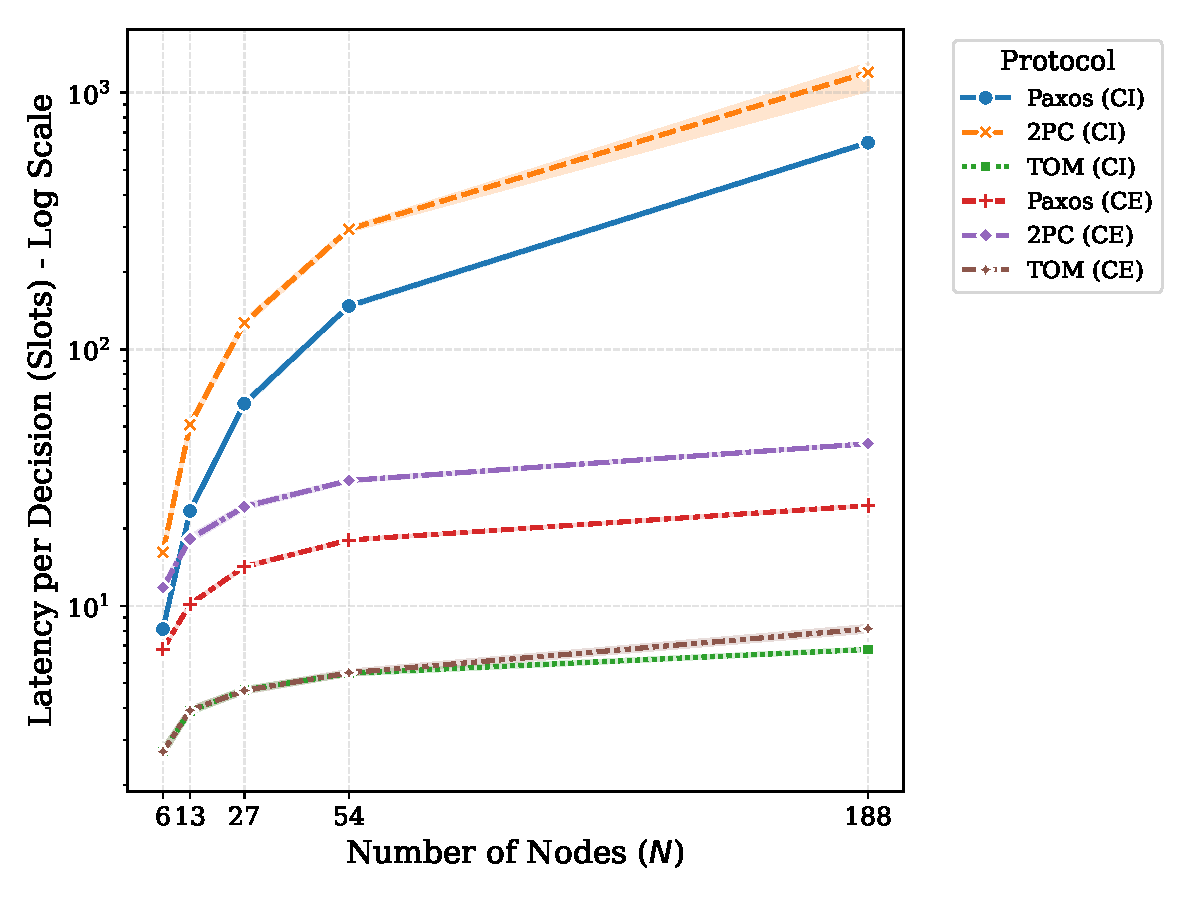
\includegraphics[width=3.4in]{latency_vs_nodes.pdf}
% \caption{Mean per-decision latency in slots (logarithmic axis) against
% network size; settings as in Fig.~\ref{fig:thr-nodes}.}
% \label{fig:lat-nodes}
% \end{figure}

Whereas Section~\ref{sec:results-throughput} measures the rate at which a
workload completes, this subsection isolates the temporal cost of a
\emph{single} decision. On a logarithmic vertical axis, latency growth
with $\Nnodes$ is close to multiplicative for the vote-based protocols
and almost flat for TOM.

The TOM family operates near the theoretical bound set by the network
diameter, at roughly 2 to 8 slots, rising only slightly with $\Nnodes$,
since each decision is nothing more than a single-phase dissemination.
Notably, the two TOM curves coincide almost exactly across the whole
range of $\Nnodes$ and separate only at $\Nnodes = 188$ (about 6.6
against 7.6 slots, this time in favour of \CI). This coincidence is
independent evidence for the analysis in
Section~\ref{sec:results-dynamics}.

Paxos and 2PC over \CE{} occupy the middle of the plot, at roughly 25 and
44 slots respectively at $\Nnodes = 188$: each decision completes within
a single goal-oriented round, but the voting rules and the two-phase
structure make that round longer than TOM's. Their growth with $\Nnodes$
is very gradual, because early termination allows each round to last only
as long as it needs to.

The highest latencies belong to the pipelined variants of Paxos and
especially 2PC. Latency for 2PC over \CI{} rises from about 170 slots at
$\Nnodes = 6$ to more than 1700 slots at $\Nnodes = 188$, and Paxos over
\CI{} from about 8 to about 620 slots. \textbf{This does not contradict
the throughput results; it complements them.} In a pipelined
architecture the lifetime of an individual decision is deliberately
stretched so that the radio schedule stays regular and flood rounds
remain shared among several proposals. High latency is therefore the
\emph{price of concurrency} rather than a symptom of a slow system:
during the interval in which one decision is waiting to complete, dozens
of others are making progress, a claim quantified in
Section~\ref{sec:results-dynamics}. The gap between 2PC and Paxos over
\CI{} is likewise expected, since unanimity demands a longer waiting
window than a majority.

The design implication is that the choice between \CI{} and \CE{} should
not be made on single-shot latency. If the application criterion is the
response deadline of an individual time-critical event, \CE{} is the
right choice for vote-based protocols; if the criterion is the completion
of a bulk workload or energy consumption
(Section~\ref{sec:results-energy}), the higher latency of \CI{} is an
acceptable price for substantially greater efficiency. For TOM the
question does not arise, since the two architectures deliver identical
latency.

%%---------------------------------------------------------------------
\subsection{Scheduling and System Dynamics}
\label{sec:results-dynamics}
% NOTE: the floats below are commented out until the vector PDFs exist.
% When uncommenting, also insert the corresponding figure cross-references into
% the prose; the text is currently written so that it reads correctly
% without them.

To characterise transient behaviour and sustained output we recorded the
cumulative progress of each combination towards 100 committed decisions,
and examine it under both a logarithmic and a linear time axis. The former
resolves the opening of the run and the latter the long-run rate; the two
together separate agility from sustained throughput. The network is the
reference configuration of $\Nnodes = 27$ nodes, random topology of
diameter 4, at 5\,\% link loss.

\subsubsection{Initial agility: what determines the time to a first
decision?}

% TODO: uncomment once figures/progress_over_time_log.pdf and
% figures/progress_over_time.pdf exist.
% Consolidated two-panel float. Panel (a) is the logarithmic view
% discussed in this subsubsection, panel (b) the linear view discussed in
% the next one. Placed at the top of the page the float serves both.
% \begin{figure}[!t]
% \centering
% \subfloat[Logarithmic time axis.]{%
%   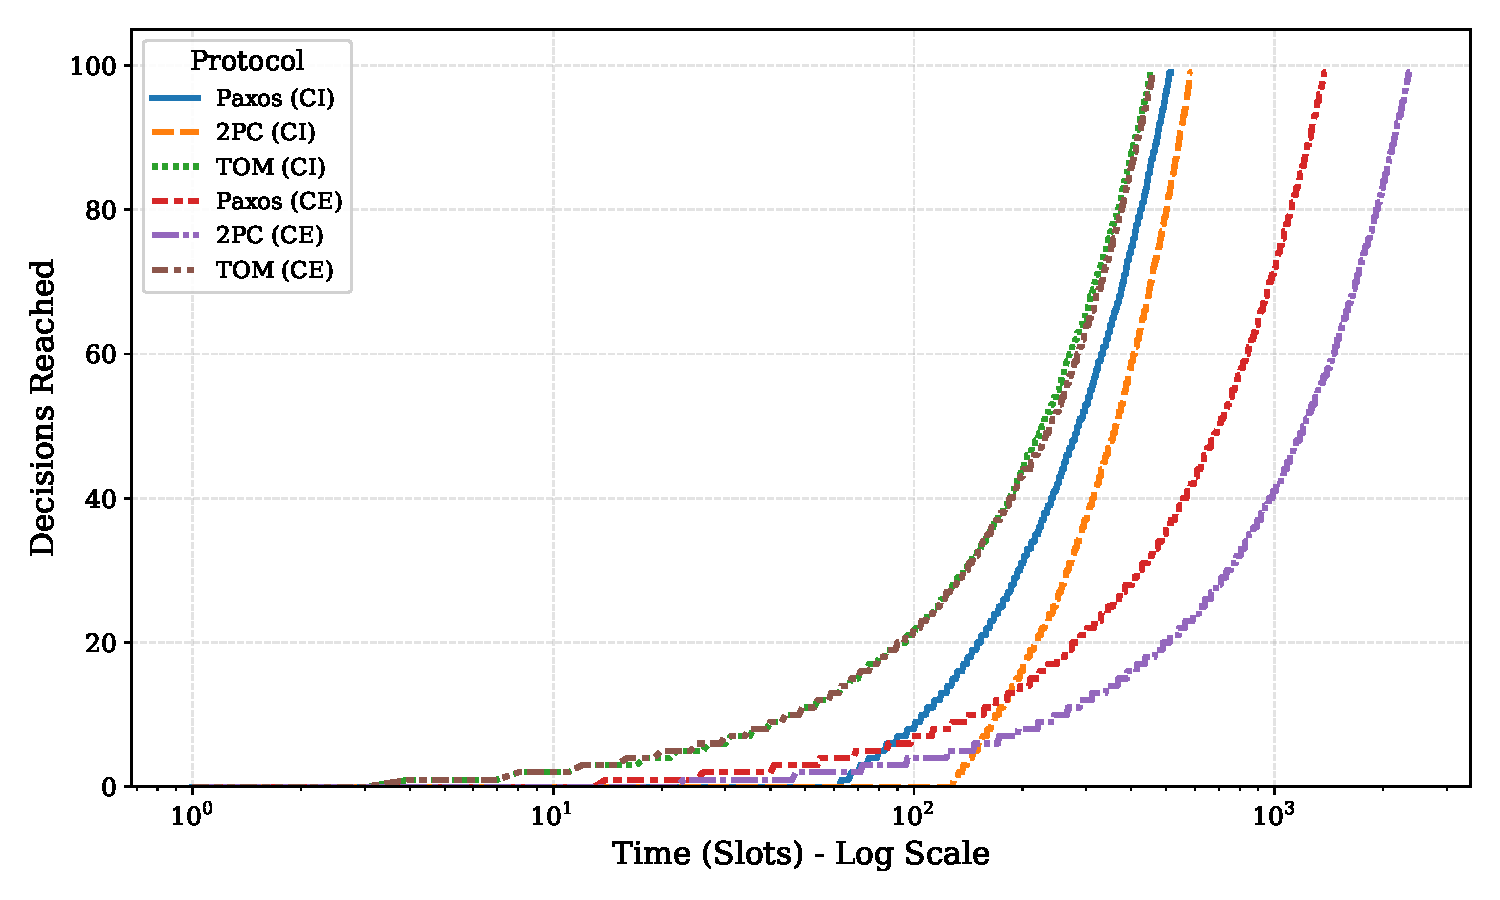
\includegraphics[width=1.65in]{progress_over_time_log.pdf}%
%   \label{fig:progress-log}}
% \hfil
% \subfloat[Linear time axis.]{%
%   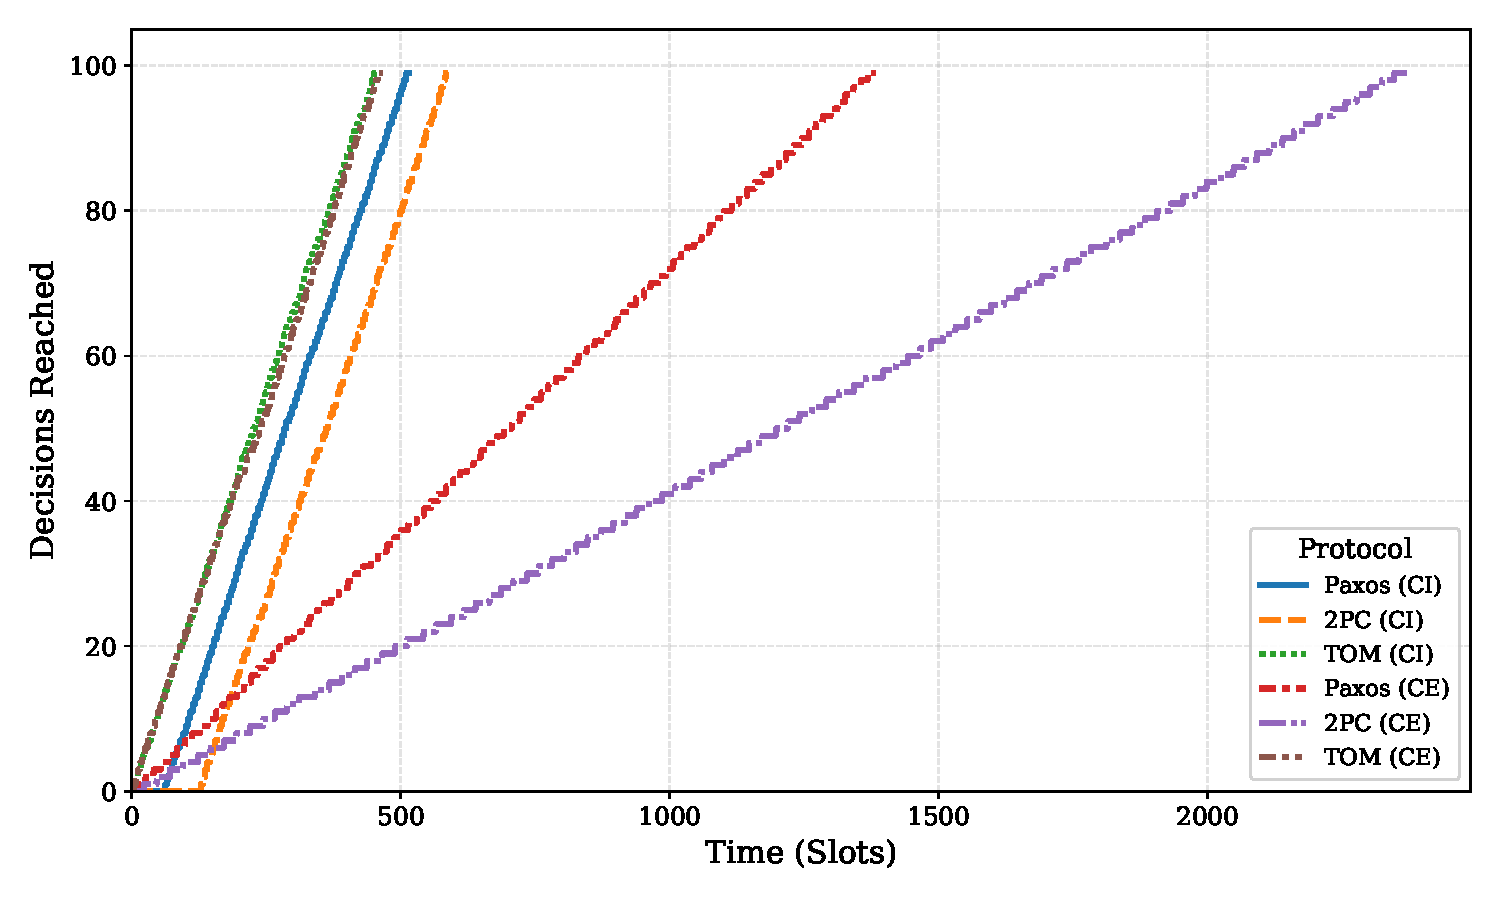
\includegraphics[width=1.65in]{progress_over_time.pdf}%
%   \label{fig:progress-lin}}
% \caption{Cumulative completed decisions against time. (a) The
% logarithmic scale resolves the opening of the run and exposes the order
% in which the combinations enter their productive phase. (b) On a linear
% scale the slope of each curve is the instantaneous decision rate and the
% intersection with 100 is the workload completion time.}
% \label{fig:progress}
% \end{figure}

The logarithmic view reveals a clear and, at first sight, unexpected
ordering. One might attribute early agility to the goal-oriented \CE{}
physical layer, since a \CE{} round terminates as soon as its goal is met.
The measurement says otherwise: what determines the time to a first
decision is the \emph{structural weight of the protocol}, not the
communication architecture. Both TOM variants begin producing decisions in
the very first slots, lie almost exactly on top of one another, and stay
ahead of every competitor throughout the opening phase---including the
\CE{} protocols. They are followed by Paxos over \CE, then 2PC over \CE,
then Paxos over \CI, and last 2PC over \CI.

The near-perfect coincidence of the two TOM curves is the key to this
plot. TOM is a single-phase dissemination and each of its decisions is
nothing more than one propagation wave. In such a structure the pipeline
has no phase available to overlap and therefore imposes no meaningful
warm-up cost; conversely, early termination under \CE{} yields no
significant advantage either, because a single-phase dissemination already
operates close to the bound set by the diameter and leaves no room for
shortening.

Pipeline warm-up is a real phenomenon, but its scope is confined to the
vote-based protocols. Paxos and especially 2PC over \CI{} produce no
definitive output in the opening slots and their progress lines stay flat,
because each decision must traverse several flood rounds to collect votes
and, until the pipeline fills, no decision satisfies the all-node
completion condition. The same plot also explains the gap between the two:
unanimity demands a longer waiting window than a majority, which delays
2PC over \CI{} more than any other combination.

The same curves show, however, that this initial deficit is short-lived.
Once the \CI{} combinations enter their productive phase they rise so
steeply that they overtake their \CE{} counterparts within a small
fraction of the total run. The conclusion is that a fast start should not
be credited to the \CE{} family at all: it is a property of lightweight,
single-phase protocols and is equally available on both substrates.

\subsubsection{Sustained throughput and the long-run outcome}

% NOTE: the linear view is panel (b) of the consolidated progress float
% placed at the start of the preceding subsubsection.

The linear view presents an almost inverted picture and shows that initial
agility is a poor predictor of workload completion time. Once warm-up
ends, the \CI{} curves climb steeply, uniformly and almost perfectly
linearly, whereas Paxos and 2PC over \CE{} advance in a slow staircase,
because each proposal requires its own exclusive round and the next
decision cannot begin until the current round ends.

The central observation is a \textbf{complete separation of the two
families}: all three \CI{} combinations finish the 100-decision workload
before either vote-based \CE{} protocol does. Even the slowest pipelined
combination---2PC over \CI, which carries the highest per-decision
latency in the entire system at nearly 360 slots---completes the workload
in about 590 slots, more than twice as fast as Paxos over \CE{} at about
1420 slots and close to four times faster than 2PC over \CE{} at about
2430 slots. This comparison alone establishes that per-decision latency
and workload completion time are independent quantities.

At the head of the ranking, TOM over \CI{} and TOM over \CE{} reach the
finish line together at about 470 slots, their curves coinciding
throughout the run, followed by Paxos over \CI{} at about 525 slots and
2PC over \CI{} at about 590. The slowest combination to reach the finish
line is 2PC over \CE: unanimity combined with strictly sequential
dissemination in the presence of 5\,\% loss requires more than five times
the time of the fastest combination in the system.

\subsubsection{Pipeline depth: quantifying concurrency and the TOM
boundary case}

The preceding analyses attributed the advantage of the pipeline to the
overlap of proposals, and the equivalence of the two architectures under
TOM to the absence of any overlappable phase. Both claims can be extracted
directly and quantitatively from the columns of
Table~\ref{tab:baseline} through Little's law,
Equation~\eqref{eq:depth}. The result is Table~\ref{tab:depth}.

\begin{table}[!t]
\caption{Effective pipeline depth, computed from Little's law
(Equation~\eqref{eq:depth}) applied to the values of
Table~\ref{tab:baseline}.}
\label{tab:depth}
\centering
\footnotesize
\begin{tabular}{@{}lrrr@{}}
\toprule
\textbf{Protocol} & \textbf{Throughput} & \textbf{Latency} &
$\boldsymbol{\Cdepth}$ \\
\midrule
TOM (\CE)   & 0.2143 & 4.7   & 1.00 \\
Paxos (\CE) & 0.0704 & 14.2  & 1.00 \\
2PC (\CE)   & 0.0412 & 24.3  & 1.00 \\
\addlinespace
TOM (\CI)   & 0.2132 & 4.7   & 1.00 \\
Paxos (\CI) & 0.1903 & 61.4  & 11.66 \\
2PC (\CI)   & 0.1681 & 126.8 & 21.25 \\
\bottomrule
\end{tabular}
\end{table}

The table settles three questions at once. First, all three \CE{}
combinations have a depth of exactly unity. This is the empirical
confirmation of the sequentiality assumed in
Section~\ref{sec:baseline-sequential}: at any instant exactly one proposal
is in flight, never more. That finding is the foundation of the structural
identity derived below.

Second, the informal claim of overlap becomes a specific number: Paxos
over \CI{} keeps about twelve proposals in flight on average and 2PC over
\CI{} about twenty-one. This is precisely how 2PC over \CI{} sustains a
throughput of 0.168 decisions per slot while each individual decision
takes 127 slots---the high latency is not slowness but the consequence of
each decision spending most of its life alongside dozens of others. It
also explains why 2PC runs deeper than Paxos: the longer waiting window
imposed by unanimity accumulates more proposals in the system
simultaneously.

Third, and most importantly, \textbf{TOM over \CI{} also has a depth of
exactly unity}. This promotes the TOM boundary case from a qualitative
interpretation to a measured fact: under TOM the pipeline carries no
concurrency whatsoever and is, in this respect, indistinguishable from
sequential execution. The reason is that TOM is not a full agreement
process with round-trip phases; when every decision is a single
propagation wave there is nothing to overlap, and the pipeline is reduced
to one message per consecutive round. Consistently with this, the
throughput of TOM over \CI{} is exactly the reciprocal of its latency
($0.213 \approx 1/4.7$): the system is \emph{latency-bound}, not
\emph{pipeline-bound}.

The significance of this boundary case is that it \emph{removes the
trade-off}. Under Paxos and 2PC, choosing \CI{} means accepting higher
per-decision latency in exchange for throughput and efficiency. Under TOM
no such price is paid: at identical pipeline depth, identical latency and
identical throughput, the \CI{} architecture still delivers markedly
better energy efficiency (2.43 against 1.70 in
Table~\ref{tab:baseline}). Since no amortisation is at work, that
advantage arises \textbf{entirely and exclusively from the ability to put
the radio to sleep} after each flood wave---a capability the baseline,
with its always-on radio, structurally lacks. TOM therefore functions as a
controlled experiment that separates the two saving mechanisms of the
\CI{} architecture: setting the amortisation term to zero leaves the pure
duty-cycling term exposed.

Finally, the equivalence in speed is confined to small and medium
networks. As Section~\ref{sec:results-throughput} showed, TOM over \CI{}
pulls away from TOM over \CE{} from $\Nnodes = 54$ onward and is about
20\,\% faster at $\Nnodes = 188$. TOM is thus not an exception to the
thesis of this paper but its simplest instance: even in the worst case for
pipelining---where there is no phase to overlap at all---the \CI{}
architecture consumes less energy at no cost in speed.

%%---------------------------------------------------------------------
\subsection{Energy Consumption}
\label{sec:results-energy}

\subsubsection{Metric: amortised per-decision energy}

A fair accounting of energy under high offered load must take into account
that in the pipelined architecture several decisions are in flight at
once, as Table~\ref{tab:depth} has just quantified. Alongside the cumulative
metric we therefore also decompose the radio cost across the decisions that
were in flight when it was incurred. This decomposition is not the basis of
any ratio reported in this paper; it exists to give the per-decision
\emph{distributions} below. For each
successful proposal $i$ with lifetime $[s_i, e_i)$,

\begin{equation}
\label{eq:amortized}
E_i \;=\; \sum_{t=s_i}^{e_i-1} \frac{A_t}{C_t} ,
\end{equation}

where $A_t$ is the number of nodes awake---listening or flooding---in slot
$t$, and $C_t$ is the number of concurrent proposals whose lifetime spans
slot $t$. The metric divides the radio cost of each slot fairly among all
proposals that the slot actually served.

\subsubsection{A structural identity: the energy ceiling of the baseline}

Before turning to numbers, one structural property of the baseline
deserves attention, because it is the key to reading every result in this
subsection. Two conditions hold simultaneously in the \CE{} protocols.
Processing is strictly sequential, so at most one proposal is in flight
and $C_t \equiv 1$---which is structural under \CE{} rather than measured.
And the radio of every node stays on
for the whole round and never sleeps, so $A_t = \Nnodes$, which the zero
Sleep column of Table~\ref{tab:baseline} confirms for all three \CE{}
combinations. Substituting both conditions into
both energy definitions collapse the per-decision energy of the baseline
onto exactly the ceiling anticipated analytically in
Equation~\eqref{eq:ece}, with $\Lround$ instantiated as the latency of the
decision; under \CE{} the cumulative and decomposed accounts coincide, so the
ceiling does not depend on which of the two is used.

This is not an empirical fit but a direct consequence of the structure of
the baseline, and the measurements confirm it closely: for TOM,
$27 \times 4.7 = 126.9$ against 126.3 measured; for Paxos,
$27 \times 14.2 = 383.4$ against 383.6; and for 2PC,
$27 \times 24.3 = 656.1$ against 657.1.

The implication runs deeper than a consistency check. In the baseline
architecture, energy and latency are two names for one quantity: every
slower decision is proportionally more expensive, and the designer has no
lever with which to separate them. The entire claim of this paper can be
stated in these terms---the pipelined \CI{} architecture breaks that
forced coupling, and it does so through two independent mechanisms:
reducing $A_t$ by sleeping the radio, and raising $C_t$ through
concurrency.

\subsubsection{Distinguishing the two energy metrics}

Two energy metrics with different purposes are reported in this paper and
the distinction between them must be explicit.

The first is the \textbf{cumulative per-decision energy}, defined as the
total number of listening and flooding slots over the whole run divided by
the number of committed decisions. It charges the entire radio cost of the
workload---including pipeline fill and drain slots---to the decisions, and
because it yields a single concurrency-independent number it is the basis
of Table~\ref{tab:baseline} and of the efficiency results below.

The second is the \textbf{amortised per-decision energy} of
Equation~\eqref{eq:amortized}, which accounts for cost only within the
lifetime of the proposal itself and only after division by the degree of
concurrency. Unlike the first, this definition produces a
\emph{distribution} over individual decisions, which is what the
distributional views below require.

The relationship between the two is instructively architecture-dependent.
Under \CE, strict sequentiality means that no slot falls outside the lifetime
of some active proposal, so the two coincide and both reduce to
$\Nnodes \cdot L$; this was verified on every one of the 4500 \CE{} decisions
measured. Under \CI{} the decomposition is smaller than the cumulative metric,
because it does not charge the decisions for the slots after the last one
commits. The gap is small and it is not a fixed overhead: $0.08\,\%$ of the
radio cost for TOM, $1.66\,\%$ for Paxos and $4.57\,\%$ for 2PC. All ratios
reported in this paper are cumulative, so no result depends on that gap.

\subsubsection{The magnitude of the reduction}

% TODO: uncomment once figures/energy_mean_ci_ce.pdf exists.
% \begin{figure}[!t]
% \centering
% 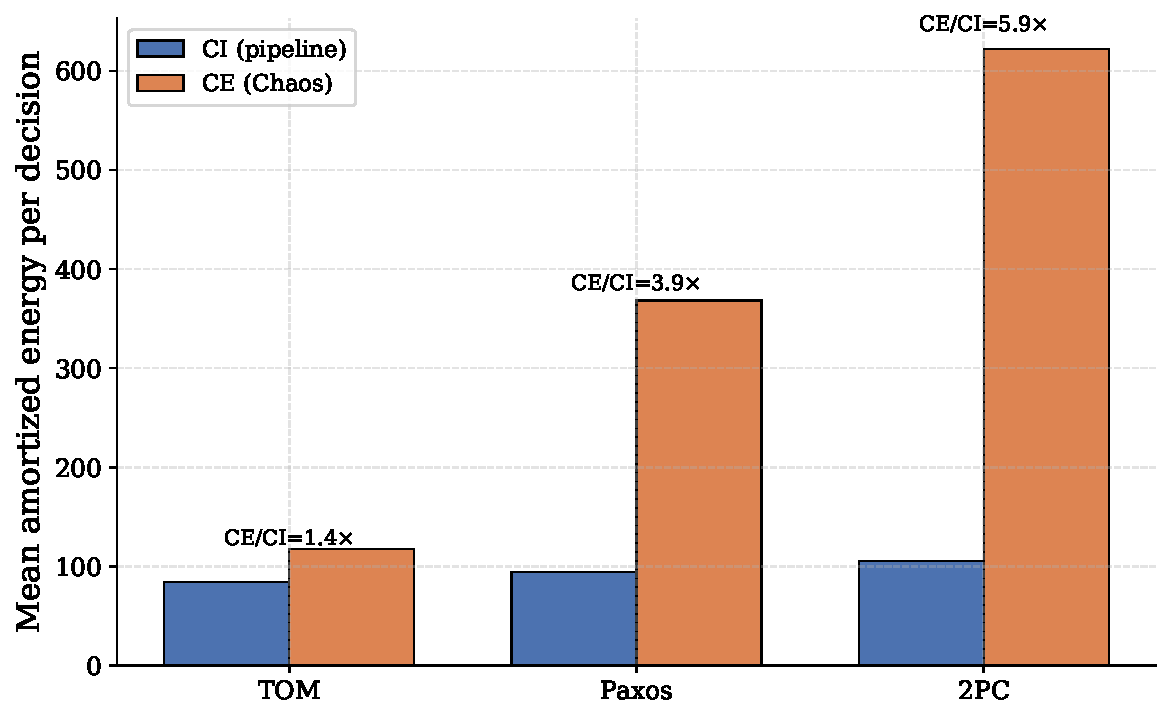
\includegraphics[width=3.4in]{energy_mean_ci_ce.pdf}
% \caption{Mean amortised energy per decision by protocol and
% architecture. The label above each pair of bars gives the ratio of the
% baseline to the pipelined variant.}
% \label{fig:energy-mean}
% \end{figure}

Under the cumulative criterion, the pipeline reduces the energy required
per final decision, relative to sequential execution of the same protocol
on the same workload, by a factor of $3.83 \pm 0.07$ for Paxos and
$5.67 \pm 0.27$ for 2PC (95\,\% intervals over fifteen seeds).

The ascending order of these ratios---$1.43 \pm 0.02$ for TOM, $3.83$ for
Paxos and $5.67$ for 2PC---is informative in itself. The heavier the protocol
and the longer its waiting window, the more slots each decision occupies and
the deeper the pipeline runs. At the low end of that spectrum sits TOM with
unit depth, where the $1.43$-fold saving arises \textbf{entirely from duty
cycling}: the measured radio duty cycle of $0.69$ predicts $1/0.69 = 1.443$,
which accounts for the measured ratio to within $0.6\,\%$. The number $1.43$
therefore marks the floor of the saving offered by the \CI{} architecture---the
part available even in the complete absence of concurrency. The rise from there
to $5.67$ under 2PC is not proposal sharing, which accounts for $1.6\,\%$ of
it; it is the number of slots a decision occupies, measured as total simulated
slots per committed decision and summed over seeds, which runs from $4.70$ to
$6.17$ under \CI{} against $4.68$ to $24.34$ under \CE.

It must be stressed that this advantage is \textbf{intra-protocol} and
does not amount to a claim that \CI{} dominates \CE{} across protocols.
TOM over \CE, at roughly 126, remains cheaper than either Paxos or 2PC
over \CE, because the intrinsic simplicity of TOM---single-phase
dissemination against multi-phase agreement---is an independent factor of
comparable weight to the communication architecture. The choice of a heavy
protocol cannot be compensated for by pipelining alone.

% TODO: uncomment once figures/energy_boxplot.pdf exists.
% \begin{figure}[!t]
% \centering
% 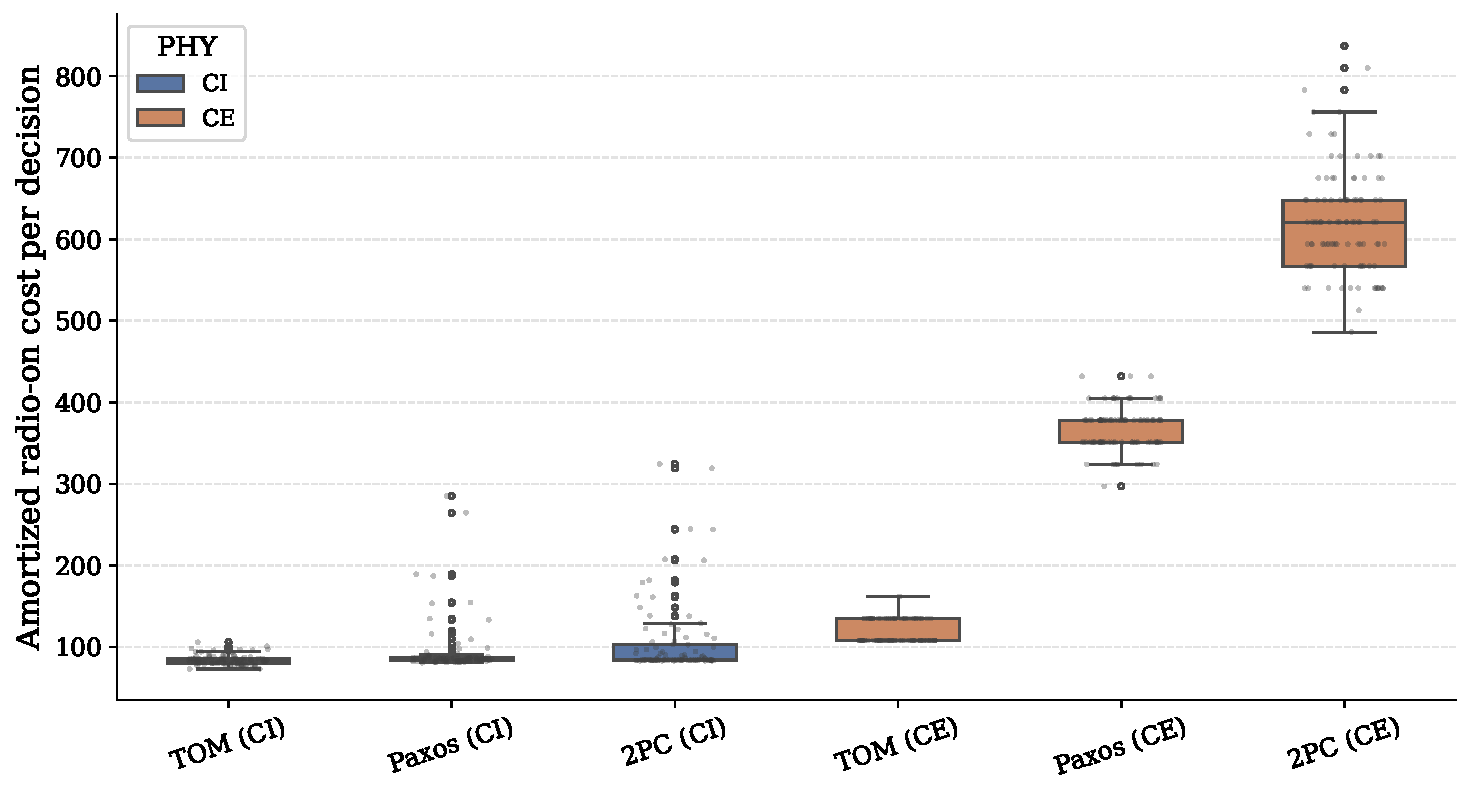
\includegraphics[width=3.4in]{energy_boxplot.pdf}
% \caption{Distribution and spread of radio-on cost per decision. Boxes
% show the median and interquartile range; points show individual
% proposals.}
% \label{fig:energy-box}
% \end{figure}

The distributional view adds two further observations. First, the \CI{} and
the vote-based \CE{} families occupy separate regions of the cost axis: the
upper quartile of the pooled \CI{} decisions lies at 94.5 node-slots and the
lower quartile of Paxos over \CE{} at 351, a factor of $3.7$ apart with no
interquartile overlap, and the $99$th percentile of the pooled \CI{}
decisions, 269.9, still lies below the $1$st percentile of Paxos over \CE,
324.0. The extreme tails do meet---the most expensive \CI{} decision observed
costs 369.3 against 297.0 for the cheapest Paxos decision over \CE---so the
separation is a statement about the bulk of the distributions and not about
their extremes. TOM over \CE{} occupies an intermediate position, its median
decision costing 135 node-slots, above every \CI{} median and far below the
two vote-based \CE{} protocols; that median is exactly $\Nnodes$ times the
median \CE{} latency of 5 slots.

Second, the three \CI{} combinations are ordered by median cost---87.0 for
TOM, 89.0 for Paxos, 90.6 for 2PC---while their concurrency spans a factor of
twenty-one, and the cost of that concurrency lands in the upper tail rather
than in the box: the $99$th percentiles run 109.0, 269.5 and 334.5. The three
distributions interleave at the bottom, the $1$st percentile of 2PC over \CI{}
at 83.5 falling inside the interquartile range of TOM, and separate at the top.
Spread is not monotone in concurrency---Paxos carries eleven times TOM's
concurrency in a narrower interquartile range, 7.2 against 9.0---so it is the
median and the upper percentile, not the width of the box, that measure what
the pipeline costs. This is the decoupling in its per-decision form: mean
concurrency rises from 1.00 to 20.84 while the median cost of a decision rises
by $4.2\,\%$.

% NOTE: the separate energy-histogram float was removed during figure
% consolidation. The multimodal structure it showed is described in the
% prose below and is also visible in the boxplot above; restore the float
% only if a reviewer asks for it.

A frequency view of the same data brings out the multimodal structure of
the distribution: the bulk of the \CI{} decisions falls in the cheapest
bins, below 100; TOM over \CE{} sits coherently between 100 and 150; and
Paxos and 2PC over \CE{} lie in the expensive bins above 300, with less than
$1\,\%$ of the \CI{} family overlapping them.

\subsubsection{Divergence of latency and energy}

% TODO: uncomment once figures/latency_vs_energy.pdf exists.
% \begin{figure}[!t]
% \centering
% 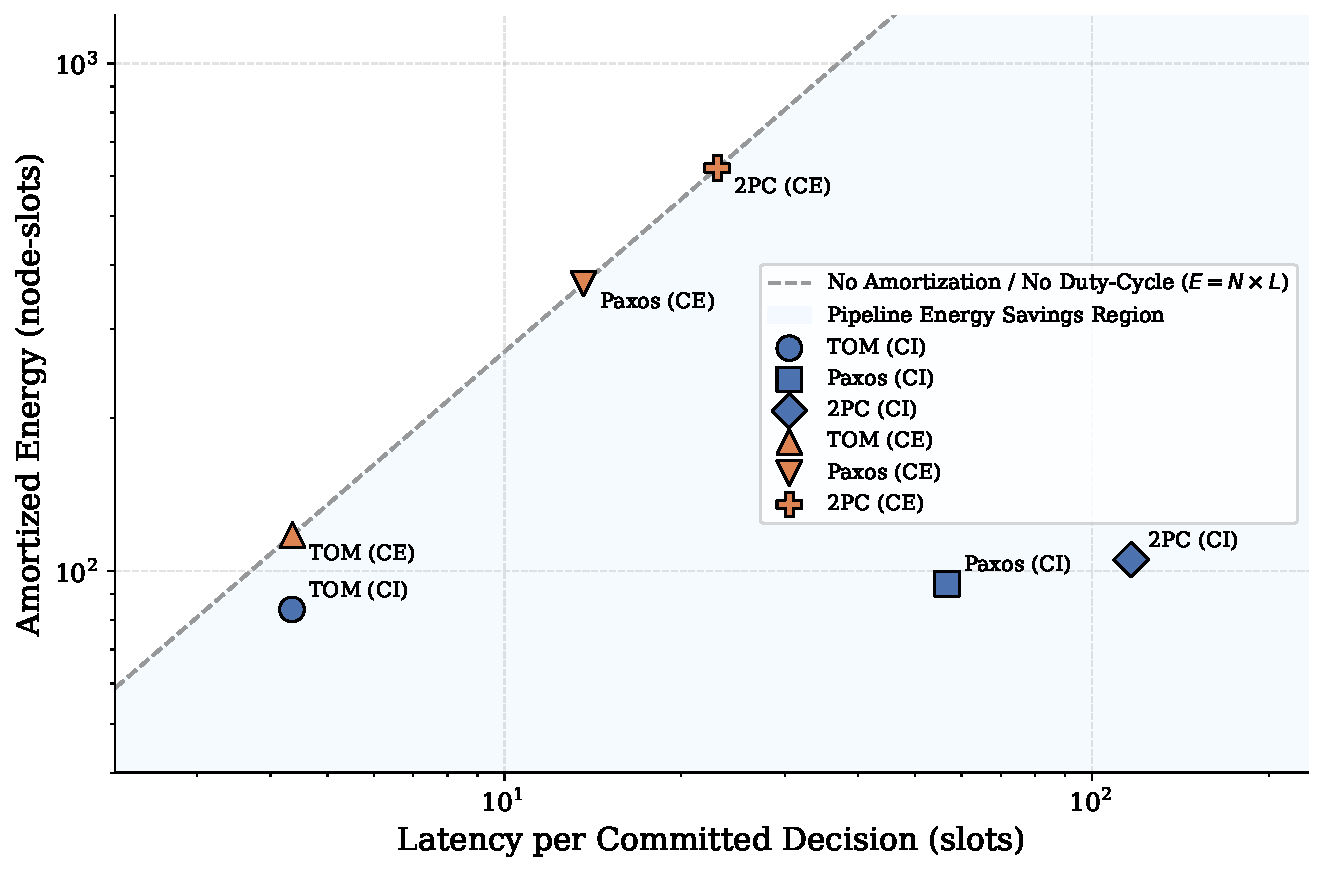
\includegraphics[width=3.4in]{latency_vs_energy.pdf}
% \caption{The latency--energy trade-off. Each point is one
% protocol\,$\times$\,architecture combination. The dashed reference line
% is the identity of Equation~\eqref{eq:ece}, that is, the behaviour of a
% hypothetical system with neither amortisation nor duty cycling. The
% shaded region below it is the energy-saving space reachable only by
% pipelining.}
% \label{fig:lat-energy}
% \end{figure}

The latency--energy plane summarises the main conceptual result of this
evaluation in a single picture. The three baseline points lie on the
reference line of Equation~\eqref{eq:ece}---not approximately but
exactly, since that line expresses a structural identity for sequential
processing with an always-on radio. The baseline architecture is
\textbf{pinned} to the line and has no degree of freedom with which to
escape it.

All three \CI{} points, by contrast, lie appreciably below the line, and
their vertical distance from it grows sharply with latency.
Table~\ref{tab:escape} quantifies the effect.

\begin{table}[!t]
\caption{Distance of the pipelined combinations from the structural
energy ceiling of the baseline. Energy is cumulative per-decision energy
averaged over fifteen seeds.}
\label{tab:escape}
\centering
\footnotesize
\setlength{\tabcolsep}{4pt}
\begin{tabular}{@{}lrrrr@{}}
\toprule
\textbf{Combination} & \textbf{Latency $L$} &
\textbf{Amortised $E$} & \textbf{Ceiling $\Nnodes L$} &
\textbf{Escape} \\
\midrule
TOM (\CI)   & 4.7   & 88.0  & 127  & $1.4\times$ \\
Paxos (\CI) & 61.4  & 100.2 & 1658 & $16.5\times$ \\
2PC (\CI)   & 126.8 & 115.8 & 3424 & $29.6\times$ \\
\bottomrule
\end{tabular}
\end{table}

The central observation is that between TOM and 2PC over \CI{} the latency
column grows by roughly \textbf{27 times} while the energy
column grows by only about \textbf{1.3 times}. In the pipelined
architecture, in other words, energy is very nearly
\textbf{independent of latency}. 2PC over \CI{} is the extreme case: it
sits at the far right of the plane, with a latency of about one hundred and
thirty slots, yet its energy per decision remains at the level of TOM,
the lightest protocol in the system. The reason has already been
quantified: the high latency of 2PC over \CI{} is not slowness but the
fact that each decision spent that entire interval in flight alongside
some twenty others, sharing the radio cost of every slot with them.

This reframes the trade-off that is conventionally assumed in low-power
networking. The usual expectation is that reducing latency and reducing
energy are aligned objectives---and in the baseline architecture, as the
reference line shows, they are exactly aligned. Pipelining breaks that
forced alignment and turns latency into a \textbf{design variable that can
be spent}: the designer may deliberately stretch the lifetime of each
decision so that the radio schedule stays regular and flood rounds are
shared among more proposals, and receive a substantial reduction in energy
per decision in return. Single-shot latency should therefore not be
treated as a proxy for energy consumption when low-power architectures are
compared.

\subsubsection{Scalability of energy efficiency}

% TODO: uncomment once figures/efficiency_vs_nodes.pdf exists.
% \begin{figure}[!t]
% \centering
% 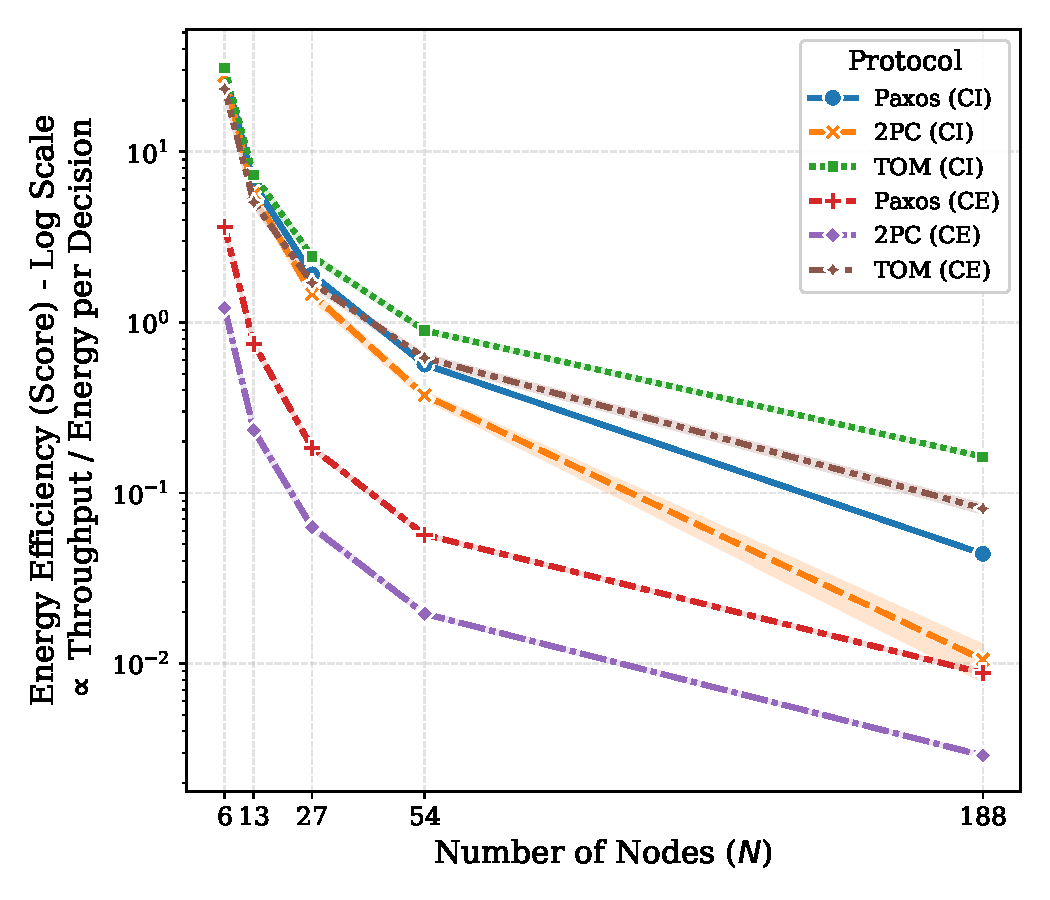
\includegraphics[width=3.4in]{efficiency_vs_nodes.pdf}
% \caption{Energy efficiency against network size (logarithmic axis,
% 5\,\% loss). Efficiency is proportional to the ratio of throughput to
% energy per decision.}
% \label{fig:eff-nodes}
% \end{figure}

The analyses above are anchored at $\Nnodes = 27$; the efficiency results
show that their conclusions survive a change of scale. Efficiency declines
for every protocol as $\Nnodes$ grows, since each decision requires radio
activity from more nodes over longer rounds. The important finding is the
\emph{stability of the intra-protocol ratios}: in all three protocol
families the \CI{} variant lies above its \CE{} counterpart at every
network size, and the gap does not close as $\Nnodes$ grows. At
$\Nnodes = 188$, Paxos over \CI{} is about five times as efficient as
Paxos over \CE, and TOM over \CI{} about twice as efficient as TOM over
\CE.

The final ranking at $\Nnodes = 188$ is

\begin{center}
TOM (\CI) $>$ TOM (\CE) $>$ Paxos (\CI) $>$ 2PC (\CI) $\gtrsim$
Paxos (\CE) $>$ 2PC (\CE).
\end{center}

TOM is thus more efficient even in its \CE{} implementation than either
pipelined vote-based protocol---an observation that again underlines the
intra-protocol nature of the advantage and shows that the
\emph{lightness of the agreement condition} is a factor of comparable
weight to the communication architecture in determining energy cost.
Notably, this ranking is itself scale-dependent: at $\Nnodes = 27$ Paxos
over \CI{} is still slightly more efficient than TOM over \CE, but from
$\Nnodes = 54$ onward TOM over \CE{} overtakes it, because the voting
overhead of Paxos grows faster with network size than the pure
dissemination cost of TOM.

%%---------------------------------------------------------------------
\subsection{Generalisation: Sensitivity to Topology}
\label{sec:results-topology}
Every analysis so far rests on a single random topology of diameter 4. It
is natural to ask whether the results---and in particular the structural
identity of Section~\ref{sec:results-energy} and the depth values of
Section~\ref{sec:results-dynamics}---are properties of that particular
graph or general properties of the two architectures. We therefore
repeated the same workload ($\Nnodes = 27$, 5\,\% link loss, 100
proposals, fifteen seeds) on the five topologies of
Table~\ref{tab:topologies}.

\begin{table}[!t]
\caption{The five topologies used in the generalisation study. All have
$\Nnodes = 27$ nodes. Mean degree is $2E/\Nnodes$ averaged over the fifteen
seeds. Diameter is a property of each generated instance rather than a fixed
input: the full mesh, partial mesh and line are deterministic, whereas the
random and scale-free generators return $\Diam = 4$ in twelve and in thirteen
of the fifteen instances respectively and $\Diam = 5$ otherwise, giving sample
means of 4.20 and 4.13. The diameters listed here are the modal values.}
\label{tab:topologies}
\centering
\footnotesize
\begin{tabular}{@{}lrr@{}}
\toprule
\textbf{Topology} & \textbf{Diameter} & \textbf{Mean degree} \\
\midrule
Full mesh    & 1  & 26.00 \\
Partial mesh & 3  & 9.30 \\
Random       & 4  & 4.40 \\
Scale-free   & 4  & 3.78 \\
Line         & 26 & 1.93 \\
\bottomrule
\end{tabular}
\end{table}

The selection is deliberate. The full mesh and the line fix the two
extremes of the design space. The random and scale-free graphs share a
diameter of 4 but have very different degree distributions, which makes it
possible to separate the effect of \emph{diameter} from the effect of
\emph{connectivity structure}---an experiment that yields an unexpected
result below.

One remark on the energy metric is needed before the results. Every energy
ratio in this paper, here and above, is the \emph{cumulative} metric of
Section~\ref{sec:results-energy}, the same quantity reported in
Table~\ref{tab:baseline}. The per-decision decomposition of
Equation~\eqref{eq:amortized} is used only for the per-decision
distributions of Section~\ref{sec:results-energy}; it is smaller than the cumulative
metric by $0.08\,\%$ for TOM, $1.66\,\%$ for Paxos and $4.57\,\%$ for 2PC,
and no ratio reported anywhere in this paper is corrected by it.

\subsubsection{Effect of diameter: who benefits from a better network?}

% TODO: uncomment once figures/throughput_vs_topology.pdf and
% figures/latency_vs_topology.pdf exist.
% Consolidated two-panel float replacing the separate throughput and
% latency figures.
% \begin{figure}[!t]
% \centering
% \subfloat[Throughput.]{%
%   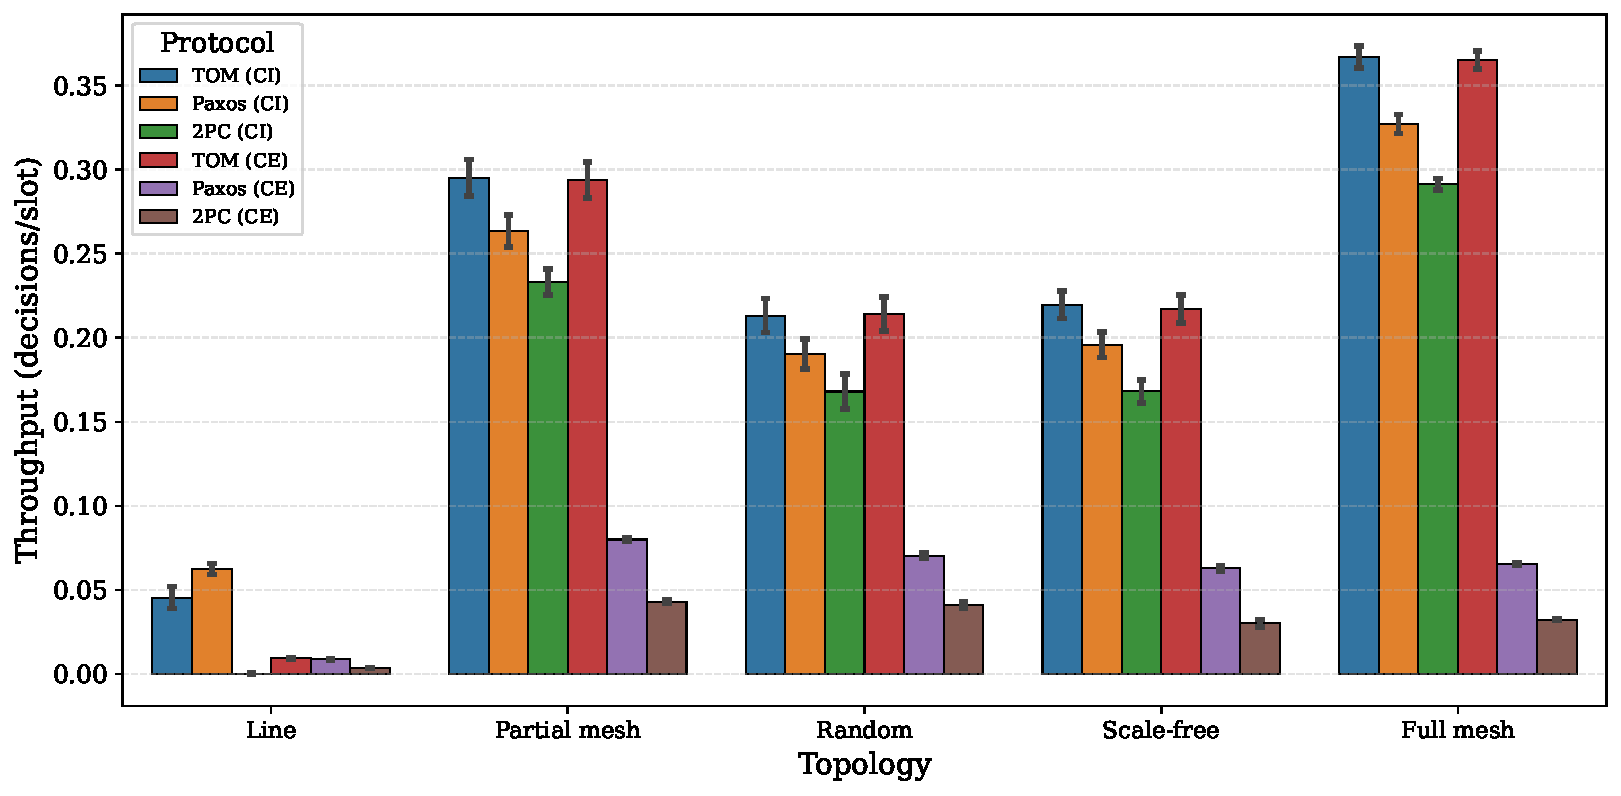
\includegraphics[width=1.65in]{throughput_vs_topology.pdf}%
%   \label{fig:thr-topo}}
% \hfil
% \subfloat[Per-decision latency, logarithmic axis.]{%
%   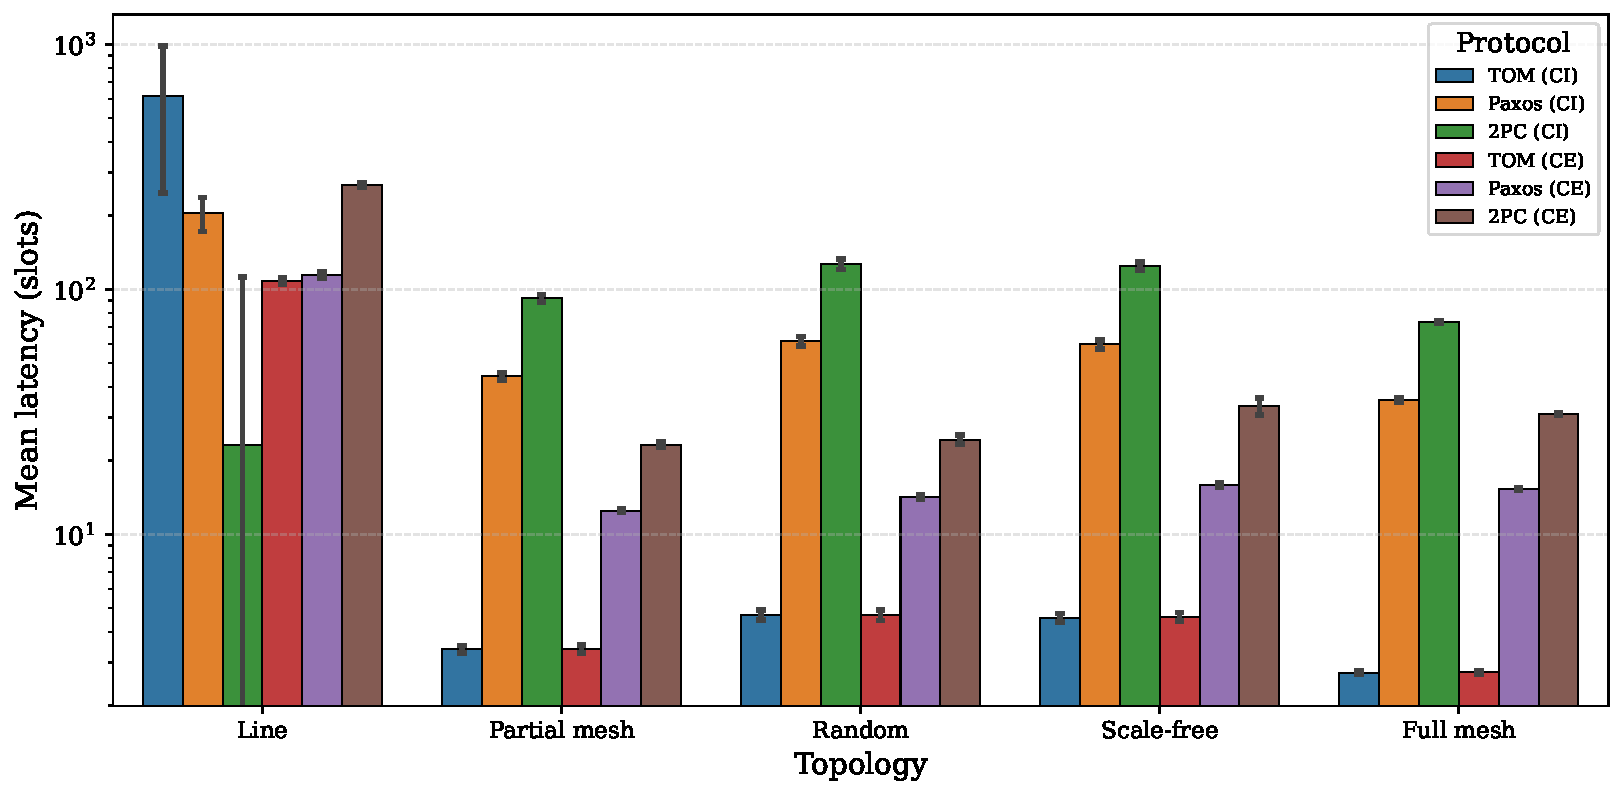
\includegraphics[width=1.65in]{latency_vs_topology.pdf}%
%   \label{fig:lat-topo}}
% \caption{Throughput and mean per-decision latency by topology and
% protocol ($\Nnodes = 27$, 5\,\% loss, 100 proposals; error bars give
% the standard error over fifteen seeds).}
% \label{fig:topology}
% \end{figure}

The proposed explanation that denser or better-quality networks account for
the residual is falsified: density error has no systematic trend with
$\Nnodes$, while both \CE{} arms remain \texttt{SUBLINEAR-INTERMEDIATE}.
Consequently, the measurements do not support attributing either the
architecture-level difference or its residual to infrastructure quality.

\begin{table}[!t]
\caption{Change in throughput on moving from the random topology
($\Diam = 4$) to the full mesh ($\Diam = 1$).}
\label{tab:diameter}
\centering
\footnotesize
\begin{tabular}{@{}lrrr@{}}
\toprule
\textbf{Protocol} & \textbf{Random} & \textbf{Full mesh} &
\textbf{Change} \\
\midrule
TOM (\CI)   & 0.213 & 0.367 & $+72$\,\% \\
Paxos (\CI) & 0.190 & 0.327 & $+72$\,\% \\
2PC (\CI)   & 0.168 & 0.291 & $+73$\,\% \\
\addlinespace
TOM (\CE)   & 0.214 & 0.365 & $+70$\,\% \\
Paxos (\CE) & 0.070 & 0.065 & $-7$\,\% \\
2PC (\CE)   & 0.041 & 0.032 & $-21$\,\% \\
\bottomrule
\end{tabular}
\end{table}

The result is striking: \textbf{Paxos and 2PC over \CE{} gain nothing
from the complete elimination of the routing problem, and in fact get
worse.} The latency measurements identify the cause. The latency of Paxos
over \CE{} is essentially constant across the four dense topologies,
between 12.5 and 15.9 slots, and is almost indifferent to the diameter
falling from 4 to 1. These protocols are, precisely speaking,
\emph{overhead-bound} rather than \emph{propagation-bound}: the fixed cost
of the goal-oriented round structure---listen timeouts, voting phases,
synchronisation---so dominates propagation time that an improvement in the
network disappears behind it. And since throughput in a sequential
architecture is nothing but the reciprocal of latency, a consequence of
$\Cdepth = 1$ established in Section~\ref{sec:results-dynamics}, constant
latency translates directly into constant throughput.

All three \CI{} protocols, by contrast, convert network quality into
throughput at an almost identical rate of about 72\,\%, because the length
of a flood round in that architecture is a direct function of the
diameter, as Equation~\eqref{eq:round} states: a shorter diameter
immediately yields shorter rounds and therefore more decisions per unit of
time. TOM over \CE{} obeys the same rule ($+70$\,\%) because it is a pure
dissemination with no voting phase to impose a fixed overhead.

These topology comparisons describe protocol sensitivity within the
committed cases, not the cause of the residual. Because the densification
hypothesis is falsified, they do not justify the broader claim that
infrastructure investment explains the architecture-level performance gap.

One further fact is established across all four dense topologies: the
agreement of TOM over \CI{} and TOM over \CE{} is remarkably stable. The
values are 0.367 against 0.365 in the full mesh, 0.295 against 0.294 in
the partial mesh, 0.213 against 0.214 in the random graph, and 0.219
against 0.220 in the scale-free graph; in no case does the difference
exceed one per cent. The TOM boundary case analysed in
Section~\ref{sec:results-dynamics} is therefore not an artefact of one
topology but a structural property.

\subsubsection{Validating the energy identity across the topology space}

% NOTE: the separate energy-versus-topology float was removed during
% figure consolidation. The identity is carried by the table below and
% the CI/CE ratios by the prose.

Equation~\eqref{eq:ece} claims that under \CE{} the energy of a decision
is exactly the product of the network size and the latency of that
decision. The claim is not open to measurement error: if the radio never
sleeps, each of the $\Nnodes$ nodes is awake in each of the $L$ slots a
decision occupies, so the product is what the accounting computes. What can be
checked is the instrument, and it holds throughout the topology space---three
\CE{} protocols on five topologies, a twenty-six-fold range of diameter and a
ninety-sevenfold range of energy per decision.

The check is on the instrument rather than on the arithmetic: the per-node
radio counters sum to $\Nnodes$ times the slots ticked in all $2250$ runs of
the study, and measured energy per decision agrees with $\Nnodes \cdot L$ to
the last bit the simulator represents. The identity is moreover visible per
decision and not only in aggregate: every one of the $4500$ \CE{} per-decision
energies measured at the reference point is an integer multiple of $\Nnodes$,
so the \CE{} per-decision energy distribution is the latency distribution
rescaled by $\Nnodes$. No \CI{} arm has that property---the per-decision
energies of Paxos and 2PC over \CI{} are in general not integers, because a
slot shared between $k$ decisions contributes $1/k$ to each.

What the check licenses is the stronger reading. It establishes
$\Ece = \Nnodes L$ as a \textbf{structural law} of the \CE{} architecture: as
long as the communication mechanism is sequential and the radio never sleeps,
the energy of a decision is locked to its latency regardless of the structure
of the network, and the designer has no lever at all---neither a better
topology nor a different protocol---with which to break that coupling. Every
departure from the law is then attributable to sleep alone, and the size of the
departure measures what pipelining buys: under \CI{} the same accounting
falls short of $\Nnodes L$ by between 22 and 31\,\% on the dense topologies,
which is exactly the fraction of node-slots those protocols spend with the
radio off. The one departure visible in the \CE{} measurements themselves is
not energy at all: where a configuration leaves a proposal uncommitted, energy
per decision exceeds $\Nnodes \bar{L}$ by $1/d - 1$, where $d$ is the measured
pipeline depth. That residual is zero to machine precision in fourteen of the
fifteen groups and reaches $1.94\,\%$ on a single seed of 2PC over \CE{} on the
line topology, where two of the fifteen seeds commit 99 proposals of 100.

On the other side, the \CI{} architecture consumes less energy than its
\CE{} counterpart for all three protocols on all five topologies. The
margin ranges between 1.3 and 12 times on the dense topologies and, worth
noting, reaches its largest value for TOM on the line, at 2916 against 401
---more than seven times. The worse the network and the longer the rounds,
the heavier the penalty imposed by an always-on radio and the greater the
value of being able to sleep.

\subsubsection{Invariance of pipeline depth}

Applying Little's law, Equation~\eqref{eq:depth}, to the data of all five
topologies produces what may be the most important finding of this
subsection. Across the four dense topologies the diameter varies by a
factor of four and throughput by a factor of about 1.7, yet
\textbf{the pipeline depth remains effectively unchanged}: TOM over \CI{}
stays at unity, Paxos over \CI{} at about 11.6 and 2PC over \CI{} at about
twenty-one in every case.

This invariance shows that the pipeline depth is an
\emph{architectural design parameter} and not a network accident. The
pipeline structurally holds a certain number of proposals in flight, and
the topology determines only how long each of them takes---not how many
there are. In practical terms this answers the question of whether the
energy savings reported in Section~\ref{sec:results-energy} depend on a
particular network: they do not, because the mechanism that generates them
is insensitive to topology.

The \CE{} columns likewise repeat a depth of exactly unity in all four
topologies, giving the assumption $C_t \equiv 1$---on which the identity
above rests---twelve further independent confirmations. And the stable
unit depth of TOM over \CI{} across all four topologies settles the
boundary-case analysis of Section~\ref{sec:results-dynamics}: the absence
of concurrency in the TOM pipeline is not an accident but a direct
consequence of the protocol being single-phase, and it does not change
under any network structure. The line topology behaves differently and is
treated separately in Section~\ref{sec:results-limitations}.

\subsubsection{Diameter is not a sufficient statistic}

The random and scale-free topologies are matched in
diameter\footnote{Both generators return $\Diam = 4$ on the majority of the
fifteen instances---twelve of fifteen for the random graph and thirteen of
fifteen for the scale-free graph, with $\Diam = 5$ otherwise. Restricting the
comparison to the ten seeds on which both graphs have $\Diam = 4$ leaves every
conclusion of this subsection intact: 2PC over \CE{} loses 27.4\,\% of its
throughput and Paxos over \CE{} 10.6\,\%, against 26.7\,\% and 10.7\,\% over
all fifteen seeds.} and comparable in mean degree, 4.40 against 3.78, but
their degree \emph{distributions} differ in shape: the scale-free graph
concentrates its edges in a few dense hubs and leaves a long tail of
low-degree nodes, whereas the random graph is close to homogeneous. Comparing
the two therefore separates the effect of connectivity structure from the
effect of diameter, as Table~\ref{tab:degree} shows.

\begin{table}[!t]
\caption{Performance on the scale-free topology and the change relative to
the random topology of matched diameter. Reference values for the random
topology are given in Table~\ref{tab:baseline}. Throughput is in committed
decisions per slot and latency in slots per decision; each absolute figure is
the mean over fifteen seeds and each change is the mean of the fifteen
per-seed relative differences.}
\label{tab:degree}
\centering
\footnotesize
\setlength{\tabcolsep}{4pt}
\begin{tabular}{@{}lrrrr@{}}
\toprule
 & \multicolumn{2}{c}{\textbf{Throughput}} &
   \multicolumn{2}{c}{\textbf{Latency}} \\
\cmidrule(lr){2-3} \cmidrule(lr){4-5}
\textbf{Protocol} & Scale-free & Change & Scale-free & Change \\
\midrule
TOM (\CI)   & 0.2197 & $+3.0$\,\%  & 4.6   & $-2.8$\,\%  \\
Paxos (\CI) & 0.1958 & $+2.9$\,\%  & 59.6  & $-2.9$\,\%  \\
2PC (\CI)   & 0.1682 & $+0.1$\,\%  & 124.7 & $-1.6$\,\%  \\
TOM (\CE)   & 0.2170 & $+1.3$\,\%  & 4.6   & $-1.3$\,\%  \\
\addlinespace
Paxos (\CE) & 0.0629 & $-10.7$\,\% & 15.9  & $+11.9$\,\% \\
2PC (\CE)   & 0.0302 & $-26.7$\,\% & 33.3  & $+36.9$\,\% \\
\bottomrule
\end{tabular}
\end{table}

The pattern is clear. All three \CI{} protocols, and TOM over \CE, are
indifferent to within about 3\,\%, whereas the vote-based \CE{} protocols
lose substantially. A paired comparison confirms that the split is not an
artefact of seed variation: the two vote-based \CE{} protocols are slower on
the scale-free graph in every one of the fifteen seeds, whereas the \CI{}
protocols are faster on eight to eleven of them.

The mechanism lies in the interaction between early termination and the
degree distribution: the \CE{} mechanism closes a round only once its goal
has been achieved, and is therefore hostage to the most weakly connected node
in the network. A scale-free graph has exactly such nodes in the tail of its
distribution. The instrumentation makes the mechanism directly visible. The
number of \CE{} listen timeouts recorded for 2PC rises from 337 on the random
graph to 2049 on the scale-free graph, stretching the run from 2433 to 3331
slots for the same one hundred committed decisions; for Paxos the count rises
from 5.4 to 30. The \CI{} protocols register no such timeouts at all, because
their round length is fixed in advance and no node is ever waited for.

The ordering of the damage is itself instructive and follows the strength
of the agreement condition: unanimity must wait for the votes of
\emph{all} weakly connected leaves and suffers most; a majority condition
can ignore them and is harmed only indirectly; and pure dissemination,
which collects no votes at all, even improves slightly, because the dense
hubs accelerate propagation. The \CI{} architecture, with its fixed and
predetermined flood rounds, fundamentally cannot \emph{see} that a node is
poorly connected---the same rigid structure identified in
Section~\ref{sec:results-dynamics} as the source of the warm-up delay
becomes, here, a shield against network heterogeneity.

The methodological implication reaches beyond this paper.
\textbf{In evaluating protocols that rely on early termination, reporting
the network diameter is not sufficient} and the degree distribution must
be reported explicitly, since two networks of identical diameter can
differ in outcome by up to 27\,\%. For architectures built on fixed rounds,
the diameter remains a sufficient statistic.

%%---------------------------------------------------------------------
\subsection{Limitations and Scope of Validity}
\label{sec:results-limitations}

The line topology is the extreme point of the design space: with diameter
26 in a network of 27 nodes, the two end nodes have one neighbour and every
other node has two; the path between the two ends of the network passes
through all of them. Every
protocol degrades sharply there---the throughput of TOM over \CE, for
instance, falls from 0.214 on the random topology to 0.009---but one
combination fails outright: \textbf{2PC over \CI{} reaches a commit rate of
only 0.2\,\%}, whereas the same protocol commits 100\,\% of proposals on
the full and partial meshes and 98.9\,\% on the random topology.

An examination of the internal mechanism shows that this is not a
measurement artefact but the direct consequence of a design assumption.
The pipeline window of 2PC is bounded by one pass of the round-robin
schedule, that is, by $\Nnodes$ rounds. That assumption is entirely
adequate for small-diameter topologies, where $\Diam \ll \Nnodes$, but
once the diameter approaches $\Nnodes$ a single flood wave no longer
suffices to carry every node's vote to the whole network. Since recovery
of missing votes in the present implementation proceeds only through the
gradual merging of the bitmap in subsequent floods, and not through a
dedicated retransmission of the prepare message
(Section~\ref{sec:design-2pc}), most proposals reach the time bound before
unanimity is complete and are explicitly aborted. Paxos, which requires
only a majority, is unaffected by the same constraint and operates on this
very topology at a full commit rate and a throughput of 0.0625---which
happens to be the highest value among all combinations on the line.

Two figures reported for 2PC over \CI{} on the line topology are
statistically meaningless and should not be interpreted: the energy per
decision (190\,180) and the efficiency (0.00) both result from division by
a denominator close to zero and merely restate the commit rate of
0.2\,\%.

This finding places an explicit constraint on the scope of validity of the
design: \textbf{the bound on the pipeline window must be scaled with the
diameter of the network and not merely with the number of nodes.}
Possible remedies---an $O(\Nnodes \cdot \Diam)$ bound, dedicated
retransmission of missing votes, or a larger number of flood
repetitions---have not been evaluated here and are left to future work. It
would also be misleading to generalise the limitation to the \CI{}
architecture as a whole: the problem arises at the intersection of a
unanimous agreement condition with a diameter-agnostic bound, and as the
behaviour of Paxos over \CI{} on the same topology shows, neither of those
two ingredients is sufficient on its own.

The behaviour of TOM over \CI{} on the line also deserves comment, though
it is of a different kind. Its latency reaches 616 slots where TOM over
\CE{} needs only 108---the only topology on which the two TOM curves
separate. The cause is in-order delivery within the pipeline: on a long
path, every gap left by a lost packet causes head-of-line blocking and
holds subsequent messages until the repair completes, exactly as
anticipated in Section~\ref{sec:design-tom}. The effect is visible in the
pipeline depth as well, where $\Cdepth$ for TOM over \CI{} jumps from
unity to about 26---but this is not productive concurrency, it is a queue
of waiting messages. Even in this unfavourable regime, however, the
throughput of TOM over \CI{} remains about five times that of TOM over
\CE{} and its energy per decision more than seven times lower. Head-of-line
blocking, in other words, inflates latency without destroying efficiency.

Beyond this design limitation, two further boundaries of validity have
already been stated and are collected here for the reader's convenience.
First, all results are obtained in simulation at the granularity of a
slot, and the scope of that abstraction, the direction of the bias it
introduces and the calibration procedure used to control it are set out in
Section~\ref{sec:method-validation}. Second, the fault model covers packet
loss only; crash and Byzantine behaviour are outside the scope of this
evaluation, for the reasons given in Section~\ref{sec:model-fault}.

%%---------------------------------------------------------------------
\subsection{Summary of Results}
\label{sec:results-summary}

Taken together, the experiments characterise six dimensions
simultaneously---rate, latency, resilience to loss, transient dynamics,
energy efficiency and generalisation across topology---and they compose
into a coherent picture.

Throughput declines with $\Nnodes$ for every design while per-decision
latency rises, most steeply for pipelined 2PC. Packet loss threatens
mainly the throughput of 2PC over \CI, because unanimity within a fixed
pipeline window is fragile; that instability, however, manifests
predominantly as a longer run rather than as failed transactions, since
the commit rate stays close to complete for every combination. The
cumulative progress view then shows that the high latency of \CI{} is
misleading: all three pipelined protocols finish the workload before
either vote-based \CE{} protocol.

The underlying mechanism was quantified by Little's law: the pipeline
holds about twelve proposals in flight under Paxos and about twenty-one under
2PC, while all three \CE{} protocols are confined to unit depth. That
concurrency, together with the ability to sleep the radio, reduces the
energy per decision substantially and---more importantly---breaks the
structural coupling between latency and energy that is unavoidable in the
baseline architecture.

The generalisation study shows that these results do not depend on a
particular network. The identity $\Ece = \Nnodes L$ holds exactly in fifteen
independent cases spanning a twenty-six-fold range of
diameter, and the pipeline depth is effectively constant across the four
dense topologies, so the mechanism that produces the energy saving is
architectural rather than topological. Two complementary findings show
that the advantage of \CI{} is not confined to energy: the vote-based
\CE{} protocols are overhead-bound and derive no benefit at all from a
better network, whereas \CI{} converts network quality into throughput at
about 72\,\%; and the \CI{} architecture is robust to heterogeneity in the
degree distribution, while early termination under \CE{} remains hostage
to the most weakly connected node and loses up to 27\,\% at constant
diameter. Against this, the line topology exposed a genuine design
limitation, in that the pipeline window bound of 2PC, scaled with the
number of nodes, is inadequate in networks of large diameter.

The claim of this paper can therefore be stated precisely. The proposed
pipelined architecture is not "fastest on every axis"---for single-decision
latency in vote-based protocols the baseline still leads, and in networks
of very large diameter the present bound for 2PC requires revision. It is,
rather, \textbf{the more efficient way to produce consensus decisions per
unit of radio energy}, while simultaneously delivering a steadier rate of
workload completion. For battery-powered deployments in which energy and a
sustained decision rate take priority over single-shot latency, the
trade-off is explicitly in favour of \CI.


\section{Conclusion}
\label{sec:conclusion}

This paper has shown that the sequential-processing bottleneck that
governs consensus over synchronous transmissions---the ``one decision per
round'' rule of capture-effect architectures---is not an intrinsic
property of agreement in the air, but a consequence of a choice made at
the communication layer. Replacing the unpredictable, goal-oriented
rounds of \CE{} with the deterministic, bounded flood rounds of \CI{}
allows the idea of pipelined execution to be carried, to the best of our
knowledge for the first time, into the complete logic of agreement
protocols rather than into data dissemination alone
(Section~\ref{sec:design}): a unified message format carrying a
participation bitmap, cumulative acknowledgement and NACK-driven
cascading recovery lets several decisions travel through the network at
once while a total order over them is still guaranteed.

The evaluation carries three messages. First, the pipeline produces real
and measurable concurrency---on average twelve simultaneous proposals for
Paxos and twenty-one for 2PC---and that concurrency raises throughput by up to
a factor of four and shortens workload completion by a larger factor
still, relative to the strongest baseline competitor. Second, under \CE{}
the energy of a decision is structurally locked to its latency,
Equation~\eqref{eq:ece}; pipelining severs that link and turns latency
into a currency that can be spent to buy energy efficiency. This is the
finding whose reach extends furthest beyond the three protocols studied
here, because it cautions against the widespread practice of treating
latency as a proxy for energy when low-power architectures are compared.
Third, the results are stable across the four dense topologies, not across
the full topology space. On the line topology, 2PC over \CI{} reaches a
commit rate of only 0.2\,\%, while TOM pipeline depth reaches about 26 and
latency reaches 616 slots. The boundary case of TOM nevertheless shows that
even with no productive concurrency, the duty-cycle saving of a radio that
is allowed to sleep can preserve the advantage of \CI{} without implying
universal topology stability.

An explicit account of the limits of validity
(Section~\ref{sec:results-limitations}) points to two immediate lines of
future work. The first is to scale the pipeline-window bound with the
diameter of the network rather than with the number of nodes, and to add
a dedicated retransmission path for votes that are lost, so that
unanimous protocols such as 2PC remain usable in elongated topologies.
The second is an implementation of the architecture on real
hardware---an nRF52 platform with a Bluetooth~5 physical layer, for
instance---in order to test the simulated results against genuine timing
and channel uncertainty. That step matters more here than it would for a
protocol study of the usual kind, because the behaviour of concurrent
transmissions depends strongly on the characteristics of the physical
layer \cite{baddeley20phy}, and this dependence can in turn affect the
effectiveness of the pipeline itself.

Two further directions are more open. One is an adaptive policy for
pipeline depth. The depth is at present a fixed architectural parameter,
yet the measurements indicate that the useful depth depends on both the
topology and the loss regime, so a controller that adjusts it at run time
may recover part of the throughput that 2PC loses under adverse
conditions. The other is the extension of the framework to Byzantine
fault tolerance. Recent work has begun to bring Byzantine agreement to
low-power wireless networks
\cite{goyal22reli,boehm24tinybft,liu25asyncbft}, and pipelining is in
principle orthogonal to that effort; the combination, however, raises
questions that are specific to this setting rather than being a matter of
adding signatures to the present message format. Authenticated messages
inflate the frame, which is the scarcest resource in a \CI{} round;
quorum arithmetic changes shape, so that the relation between the
participation bitmap and the decision rule has to be reconsidered; and
equivocation, the characteristic Byzantine behaviour, has no obvious
analogue in a flood in which every node is expected to transmit the same
bits, which suggests that detecting it may require mechanisms the capture
effect does not by itself provide. We regard this as the most interesting
of the questions that the present architecture leaves open.


% Appendices, if needed. Use \section to start each one.
%\appendices
%\section{Proof of the Round-Length Bound}


% Acknowledgment. Remove for double-blind submission.
%\section*{Acknowledgment}
%The authors would like to thank \ldots


%%=====================================================================
%% REFERENCES
%%
%% References live in refs.bib. Keep both files in the same folder.
%% Build: pdflatex paper -> bibtex paper -> pdflatex paper -> pdflatex paper
%%
%% IEEEabrv supplies the official IEEE abbreviations for journal and
%% conference names. Drop it if a venue asks for unabbreviated names.
%%=====================================================================
\bibliographystyle{IEEEtran}
\bibliography{IEEEabrv,refs}


% Author biographies. Most journals want these only in the camera-ready
% version, and they must be omitted for double-blind review.
%\begin{IEEEbiographynophoto}{First A. Author}
%Biography text here.
%\end{IEEEbiographynophoto}


\end{document}
